\documentclass[12pt,letterpaper]{article}

\usepackage{amsmath, amsthm, amsfonts, amssymb}
\usepackage{microtype, parskip, graphicx}
%\usepackage[comma,numbers,sort&compress]{natbib}
\usepackage[style=numeric-comp,
      backend=biber,
      bibencoding=utf8,
      maxbibnames=10,
      uniquename=init,
      giveninits=true,
      sorting=none,
      natbib=true,
      url=false,
      doi=false,
      isbn=false]{biblatex}
\usepackage[margin=1in]{geometry}
\usepackage{lineno}
\usepackage{longtable}
\usepackage{caption, subcaption, multirow, morefloats, rotating}
\usepackage{wrapfig}
\usepackage{hyperref}
\usepackage{threeparttable}

\frenchspacing


\newcommand{\beginsupplement}{
 \setcounter{section}{0}
 \renewcommand{\thesection}{S\arabic{section}}
 \setcounter{table}{0}
 \renewcommand{\thetable}{S\arabic{table}}
 \setcounter{figure}{0}
 \renewcommand{\thefigure}{S\arabic{figure}}
 \setcounter{equation}{0}
 \renewcommand{\theequation}{S\arabic{equation}}
}

% https://3d.bk.tudelft.nl/hledoux/blog/fiddling-biblatex/
%-- formatting hell for biblatex
%-- remove "In:"
\renewbibmacro{in:}{}
%-- no "quotes" around titles of chapters/article titles
\DeclareFieldFormat[article, inbook, incollection, inproceedings, misc, thesis, unpublished]
{title}{#1}
%-- no punctuation after volume
\DeclareFieldFormat[article]{volume}{ {#1} } 
%-- puts number/issue between brackets
\DeclareFieldFormat[article, inbook, incollection, inproceedings, misc, thesis, unpublished]{number}{\mkbibparens{#1}} 
%-- and then for articles directly the pages w/o any "pages" or "pp." 
\DeclareFieldFormat[article]{pages}{#1}
%-- for some types replace "pages" by "p."
\DeclareFieldFormat[inproceedings, incollection, inbook]{pages}{p. #1}

% https://tex.stackexchange.com/questions/81569/biblatex-parentheses-around-the-volume-number-of-an-article
\renewbibmacro*{volume+number+eid}{%
 \printfield{volume}%
 \printfield{number}%
 \printfield{eid}}
\DeclareFieldFormat[article]{number}{\mkbibparens{#1}}


% bibliographic information
%\bibliographystyle{abbrvnat}
%\bibliography{citations}
\addbibresource{citations.bib}






\title{How predictable is extinction? Forecasting species survival at million-year timescales}
\author{
 Smits, Peter\\
 %Department of Integrative Biology, University of California Berkeley\\
 \texttt{psmits@berkeley.edu} 
 \and
 Finnegan, Seth\\
 %Department of Integrative Biology, University of California Berkeley\\
 \texttt{sethf@berkeley.edu}
}
\date{}

\begin{document}

\begin{refsection}

\maketitle

\linenumbers{}
\modulolinenumbers[3]

\begin{abstract}
 A tenet of conservation palaeobiology is that knowledge of past extinction patterns can help us to better predict future extinctions. Although the future is unobservable, we can test the strength of this proposition by asking how well models conditioned on past observations would have predicted subsequent extinction events at different points in the geological past. To answer this question we analyze the well-sampled fossil record of Cenozoic planktonic microfossil taxa (foramanifera, radiolarians, diatoms, and calcareous nanoplankton.) For each group we examine how extinction probability varies over time as a function of species age, time of observation, current geographic range, change in geographic range, climate state, and change in climate state. Although the best-performing model includes time-varying effects and historical covariates (change in range and change in climate state) the improvement in predictive power over models with constant effects and no historical covariates is very minor. This model has an approximately 78\% median probability of correctly ranking the relative extinction risk any two randomly selected species. It performs nearly as well at out-of-sample prediction (70-80\%), implying that determinants of extinction risk have varied only modestly through time. An important caveat is that human impacts may substantially disrupt range-risk dynamics so that the future will be less predictable than it has been in the past.

 %risk assessments for extant species can be improved by examining past extinction patterns and by using palaeontological records to establish geographic range and abundance trajectories on geological timescales. 
 %We ask if, at a given point in time, how accurate are extinction risk predictions based on instantaneous geographic ranges and knowledge of past extinction/survival patterns?
 %Such suggestions prompt two key questions: (1) At a given timescale, to what extent are extinction risk trajectories deterministic (past trends are likely to continue into the future) versus Markovian (the future depends only on the present state)? (2) 
 %Our results imply that at million-year timescales extinction risk trajectories are nearly Markovian, perhaps because the processes driving geographic range changes vary on substantially shorter timescales. 
 %However, models based on present geographic ranges and past range-risk relationships are likely to be moderately successful at predicting future extinction/survival outcomes. 
 %In-sample model performance measures are approximately equal to out-of-sample performance measures (assessed with 5-fold cross-validation), suggesting that the determinants of relative extinction risk are fairly consistent throughout the Cenozoic. 
 %Our best supported model includes the historical covariates, change in geographic range and lag of global temperature, which indicates that the past improves our estimates of the present and future. 
 %We have confidence that our conclusions about our ability to predict species extinction risk in the future with similar accuracy to when we predict species extinction risk in the past because our in-sample model performance measures are approximately equal to out-of-sample performance. 
 %Including the historical covariates and allowing their effects to vary over time yields marginally better predictions than not including them. 
 %However, the improvement in predictive power by including these historical covariates is modest at best, absent at worst, and ultimately reflects the extremely stochastic nature of species extinction. 
 %Finally, we find support for species' extinction risk increases with age, though the strength of this effect varies among taxonomic groups. 
 %This effect is most pronounced in forams and radiolarians, and less pronounced in diatoms and calcareous nanoplankton. 
 %The greatest source of variance in survival probability is the timing of observation. 
 %Importantly, this result means that the time of an observation is a greater source of variation in survival probability when compared to species age. 
 %We find that including information on a species' change in geographic range size on average improves our predictions of species survival at million-year timescales. 
 %The effect of change in geographic range is much smaller than the effect of current geographic range, and highly variable through time as the effect changes sign and there are times where there is little evidence for any effect of past geographic range. 
 %These results imply that at million-year timescales geographic range trajectories are nearly Markovian, perhaps because the processes driving geographic range changes vary on substantially shorter timescales. 
 %The effect of change in geographic range on survival most likely stands for many interacting and unobserved processes which in-turn produce that species' geographic range and its affect on survival. 
 %These results reflect the difficulty of estimating species extinction, and that while including historical covariates does improve model performance, that gain is very small. 
 %The results of this study reinforce the importance of the promise of palaeontology and using the past to predict the future.
\end{abstract}

{\bf Keywords:} conservation, palaeobiology, extinction, forecasting



\section{Introduction}

The intensifying biodiversity crisis confronts conservation biologists with the difficult task of trying to predict which species are most threatened with extinction in the near future. Predicting which species will go extinct is difficult because reliable population and geographic range time series are typically known for only the past few decades in even the best-studied groups, and because few modern extinctions have been adequately documented. This has led to the suggestions that some risk assessments might be improved by incorporating palaeontological data \citep{Finnegan2015,Kiessling2016}. The fossil record preserves information about the full histories, include ultimate extinction, of thousands of lineages, and this information can help to augment the shorter-term higher-resolution data used to make risk assessments of extant taxa.

Past palaeobiological studies of extinction have frequently focused on identifying and measuring the effect of various potential predictors on extinction risk \citep{Harnik2011,Smits2015,Peters2008,Payne2007,Harnik2012,Ezard2011,Foote2006} or on how to identify or measure these effects \citep{Alroy2010a,Alroy2014,Alroy2001,Alroy2000,Alroy2000b,Foote2001}. This focus means that while we have a good understanding of which factors are strong and general determinants of extinction risk, we have less knowledge of how accurate or strong our predictions about the differences in extinction risk are. 

Here we ask how precise risk predictions based on fossil data might be. Because future extinctions are unobservable we cannot directly evaluate the ultimate performance of such predictions. However, we can address the question by taking a given point in the geological past, developing a predictive model based on extinction patterns prior to that point, and assessing the predictive performance of this model on unobserved (e.g. ``future'', from the point of view of the model) extinction/survival events.

Extinction intensity (average rate) and selectivity (difference in risk between taxa) vary through time and the relative risk of extinction exhibited by different taxonomic groups and how that risk varies over time is an important dynamic which shapes the rate and structure of extinction \citep{Payne2007,Payne2016,Ezard2011,Smits2019}. This variation also raises a question: given that extinction intensity and selectivity change over time, how accurate are our assessments based on past events likely to be when applied to the future? Putting aside the important question of how human activities will alter the determinants of future extinction risk, we can address this uncertainty by specifically including and modeling the temporal variation in extinction risk across a range of extinction intensities and selectivities.

Numerous studies have established that geographic range is one of the most important determinants of extinction risk in the fossil record, and that a species geographic range can be highly variable over geologic time \citep{Foote2007,Liow2010,Liow2007,Kiessling2013,Payne2007,Jablonski2003,Jablonski2008,Jablonski2006}. The degree to which the past can help to predict the future fates of species depends in part on the degree to which species’ geographic range trajectories are deterministic versus Markovian \citep{Liow2007,Kiessling2013,Foote2007b,Pigot2012}. In the former case, knowledge of the specific past trajectory of a species -- whether its range has expanded or contracted over a given time span -- might help to improve assessments of its current risk. In the latter case, only the current range of the species conveys useful information about its current risk, although we can still use prior extinction patterns to augment predictions by evaluating the relative extinction risk of species that had similar ranges in the past. Discriminating among these alternative models is thus very important for determining how best to incorporate fossil data in present risk assessments.

For this exercise we chose to analyze one of the best-sampled and studied fossil records -- the Cenozoic record of skeletonized marine planktonic microorganisms (Foraminifera, Radiolaria, Diatoms, and Coccolithophores). These data are readily available through the Neptune database, an online repository of species occurrences obtained through the Deep Sea Drilling Program and the Ocean Drilling Project \citep{Lazarus1994,SpencerCervato1999}. This database provides abundant samples in space and time, a high degree of temporal resolution for the entirety of the Cenozoic, and has an internally consistent taxonomic identification strategy -- as close to ideal data for this analysis as possible. The Neptune database records multiple phyla-scale taxonomic groups for over 60 million years, with incredible temporal resolution supported by the various age-models of the deep-sea cores from which the occurrences are recorded. Analyzing patterns of extinction and global occurrence at fine temporal scales means we can better elucidate how well we can predict species extinction at human-relevant scales.



\section{Materials and Methods}

\subsection{Data Specifications}

We analyzed microfossil occurrence information from the Neptune Database \url{http://www.nsb-mfn-berlin.de/nannotax} \citep{Lazarus1994,SpencerCervato1999}. This occurrence-based dataset includes calcareous nannoplankton, diatoms, foraminifera, and radiolarians.% -- these occurrences span the entire globe between 120 and 0 million years ago (Mya). 
Occurrences were filtered to include only those species with first occurrence was no more than 63 Mya. This filtering criterion excludes taxa that survived the K/Pg extinction or arose during its ecologically unusual recovery interval, and ensures that our occurrence histories fully overlap with the temperature time-series used as a potential extinction risk predictor (see below). 

All fossil occurrences were assigned to 1 My bins based on the estimated age of the fossil occurrence as listed in the Neptune Database. After binning, each taxon's geographic range was calculated for each of the 1 My bins in which it occurred. Geographic range was calculated as the maximum great circle distance on an ellipsoid (i.e. the Earth) between any two occurrences of that species; this distance was measured in kilometers. 

Average global temperature of each 1 My bin was calculated from estimates based on Magnesium/Calcium isotope ratios \citet{Cramer2011}. We use Mg/Ca rather than oxygen isotopes to avoid confounding effect of varying ice-volume -- this property is of particular importance for this analysis as polar ice-caps develop midway through the Cenozoic. Our data source, \citet{Cramer2011}, estimated temperature for every 0.1 My from 0 to 63 Mya. The temperature estimate for each 1 My interval was calculated as the mean of all estimates within that interval. 

See Section \ref{sec:data_desc} for a further explanation on how observations were temporally binned, and how our covariates were standardized and transformed prior to analysis.


%\begin{figure}[ht]
% \centering
% 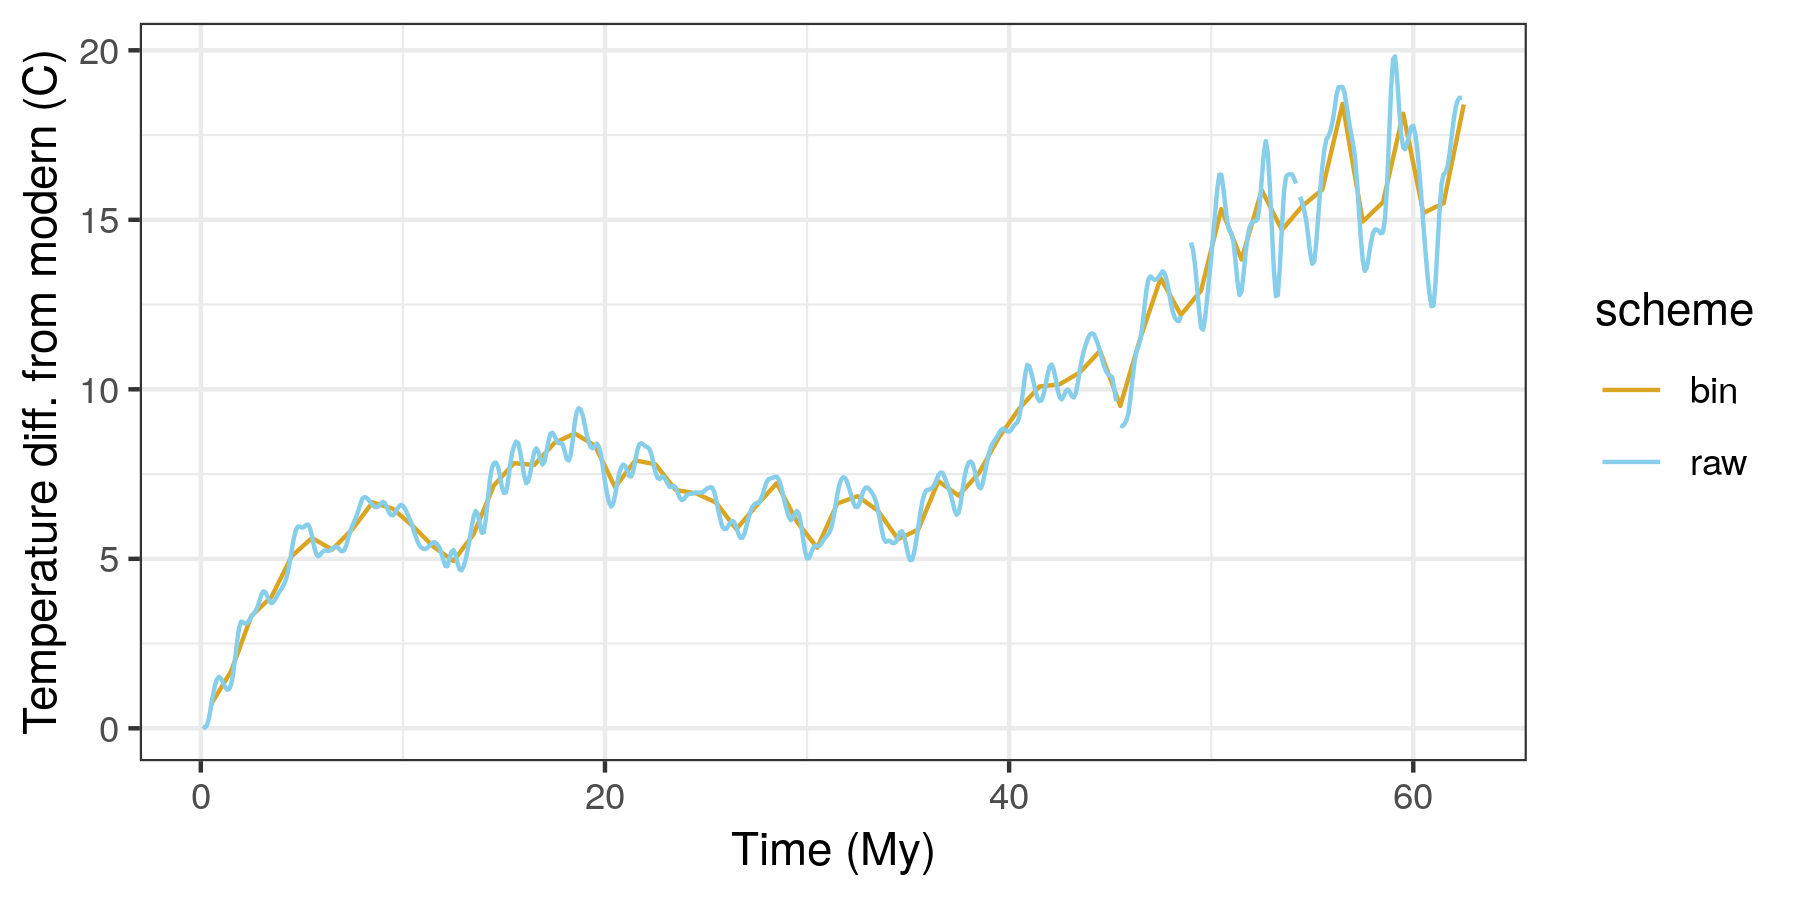
\includegraphics[width=\textwidth,height=0.5\textheight,keepaspectratio=true]{../results/figure/cramer_temp}
% \caption{Comparison of initial temperature estimates from \citet{Cramer2011} (goldenrod) versus the binned values used in this analysis (blue). The initial values are for every 0.1 My while our bins are defined for every 1 My.}
% \label{fig:temp_curve}
%\end{figure}


\subsection{Model Specifications}

We used a discrete-time survival modelling framework to estimate how well we can predict extinction risk at one million year time scales. At its core, our model is a multilevel logistic regression with taxon age in millions of years as a varying intercept \citep{Tutz2016}. We considered four different models involving different permutations of covariate effects (fixed or time-varying) and historical covariates: covariate effects constant over time and no historical covariates included (Model C), covariate effects allowed to vary over time but no historical covariates included (Model V), covariate effects constant over time and historical covariates included (Model CP), and covariate effects allowed to vary over time and historical covariates are included (Model VP). The C and P models atempt to predict based only on present state, wheras the CP and VP models allow for the possibility of non-Markovian behaviour by including change in state from the previous time increment.

We always included species age at time of observation (.e. observed prior duration) as a non-nested varying intercept term. This factor may or may not contribute to differences in species extinction risk over time \citep{Smits2015,Finnegan2008,Ezard2012,VanValen1973,Liow2011,Crampton2016}, but its inclusion in our model is critical to its nature as a survival model \cite{Tutz2016}.

See Table \ref{tab:model_def} for further explanation of how the four models we considered differ from each other. A complete description of the statistical model used in this analysis is available in Section \ref{sec:model_desc}. Additionally, the full description of how these models were implemented and coded, including choice of priors, is available Section \ref{sec:model_est}.


\begin{table}[ht]
 \caption{Models and their definitions}
 \begin{threeparttable}
  {
   \def\arraystretch{1.5}
   \begin{tabular}{ l p{3cm} l l }
    Code & Description & Covariates & R Formula Syntax\tnote{a}\phantom{\textsuperscript{a}} \\
    \hline
    C & Constant effects, no historical cov. & \parbox[t]{0.25\textwidth}{Geographic range,\\temperature} & \parbox[t]{0.33\textwidth}{event\tnote{b}\phantom{\textsuperscript{b}} $\sim$ range\tnote{c}\phantom{\textsuperscript{c}} + temp\tnote{d}\phantom{\textsuperscript{d}} +\\(1 $|$ age\tnote{e}\phantom{\textsuperscript{e}}/phylum\tnote{f}\phantom{\textsuperscript{f}})} \\
    V & Varying effects, no historical cov. & \parbox[t]{0.25\textwidth}{Geographic range,\\temperature} & \parbox[t]{0.33\textwidth}{event $\sim$ range + temp +\\(1 + range + temp $|$ phylum) + (1 $|$ age/phylum)} \\ 
    CP & Constant effects, historical cov. & \parbox[t]{0.25\textwidth}{Geographic range,\\change in geographic range, temperature,\\previous temperature} & \parbox[t]{0.33\textwidth}{event $\sim$ range + range\_diff\tnote{g}\phantom{\textsuperscript{g}} +\\temp + temp\_lag\tnote{h}\phantom{\textsuperscript{h}} +\\(1 $|$ age/phylum)} \\
    VP & Varying effects, historical cov. & \parbox[t]{0.25\textwidth}{Geographic range,\\change in geographic range, temperature,\\previous temperature} & \parbox[t]{0.33\textwidth}{event $\sim$ range + range\_diff +\\temp + temp\_lag +\\(1 + range + range\_diff +\\temp + temp\_lag $|$ phylum) +\\(1 $|$ age/phylum)} \\
    \hline
   \end{tabular}
  }
  \begin{tablenotes}
  \item[a] See Equation \ref{eq:model} for full statistical model definition.
  \item[b] Species observation where 1 if time of last observation, otherwise 0.
  \item[c] Species geographic range in log km\(^2\). Mean centered, scaled to sd = 1.
  \item[d] Global temperature in degrees C. Mean centered, scaled to sd = 1.
  \item[e] Species are at observation in millions of years.
  \item[f] Taxonomic group of species (i.e. Foraminifera, Diatoms, Radiolarians, Calcareous nannoplankton).
  \item[g] Change in geographic range since last observation.
  \item[h] Temperature at previous observation.
  \end{tablenotes}
 \end{threeparttable}
 \label{tab:model_def}
\end{table}


\subsection{In-sample and out-of-sample forecasting}

We are interested in our models' performance in two contexts: in-sample performance, and out-of-sample predictive performance (i.e. forecasting). 

In-sample forecasting means we are estimating how well our model predicts extinction probability for observations that that model was fit to. This is a posterior predictive check in that we are comparing the posterior predictive distribution to our observed data. In-sample forecasting measures, however, are not necessarily good estimates of the model's ability to predict data from the future \citep{ESL}. 

We are particularly interested in understanding how well our model forecasts extinction probability of data from the future that the model was not fit to (out-of-sample data). To quantify our ability to forecast species' extinction risk, we estimated average out-of-sample forecasting performance using 5-fold time-series cross-validation. For time-series data, the folds (data partitions) are approximately equal segments of time. Each fold represents a sequence of time points. With 63 time points, each of the five folds represents approximately 13 million-year time increments. It is important to bear in mind, however, that each time increment includes many (100s-1000s) individual observations.

k-fold cross-validation for time series follows a specific sequence of procedures \citep{Arlot2010,Bergmeir2016}. First, the model is fit to the first fold (time segment), and the posterior estimates of that fit are then used to forecast the extinction probability of the second fold (i.e. the future). Then the model is fit to the combined first and second folds, and the posterior estimates of that fit are used to forecast the extinction probability of the third fold. Continuing, the model is then fit to the first three folds combined and is then used to forecast extinction probabilities for the fourth fold. Finally, the model is fit to the first four folds combined and then is used to forecast the fifth fold. The results from these forecasts are then combined to yield our estimate of expected out-of-sample performance.

The relative adequacy of the four model variants was compared using the area under the receiver operating characteristic curve or AUC \citep{Fawcett2006,Mason2002}. This measure is commonly used to measure the performance of classification models as it has the desirable characteristic of comparing the model's true positive rate with its false positive rate, as opposed to accuracy which only considers true positives. AUC ranges between 0.5 and 1, with 0.5 indicating no difference in classification from random and 1 indicating perfect classification. AUC can be interpreted as the probability that our model correctly ranks the relative extinction risks of a randomly selected extinct-extant species pair \citep{Fawcett2006,Mason2002}. AUC values of approximately 0.8 or greater can be considered ``good'' \citep{ACCDA}, so we interpret values between 0.7 and 0.8 could then be considered ``fair,'' and values between 0.6 and 0.7 as ``poor.''

%The differences in in-sample predictive performance between the models was visualized in multiple ways: whole data set by model, taxonomic group by model, model performance over time, and model performance by taxonomic groups over time. These comparisons demonstrate the relative and absolute adequacy of the models in describing the dataset they were fit to.

See our code repository at https://github.com/psmits/trident for full code details. This entire analysis was coded in R and uses tidyverse and tidyverse adjacent tools such as \texttt{dplyr} \citep{dplyr}, \texttt{purr} \citep{purrr}, and \texttt{tidybayes} \citep{tidybayes}. Additionally, all of our models were written using the \texttt{brms} \citep{brms2017,brms2018} R package, which implements Stan-based Bayesian models which are fit via Hamiltonian Monte Carlo \citep{StanManual}.


\section{Results}

% ROC model comparison
\begin{figure}[ht]
 \begin{subfigure}[ht]{0.45\textwidth}
  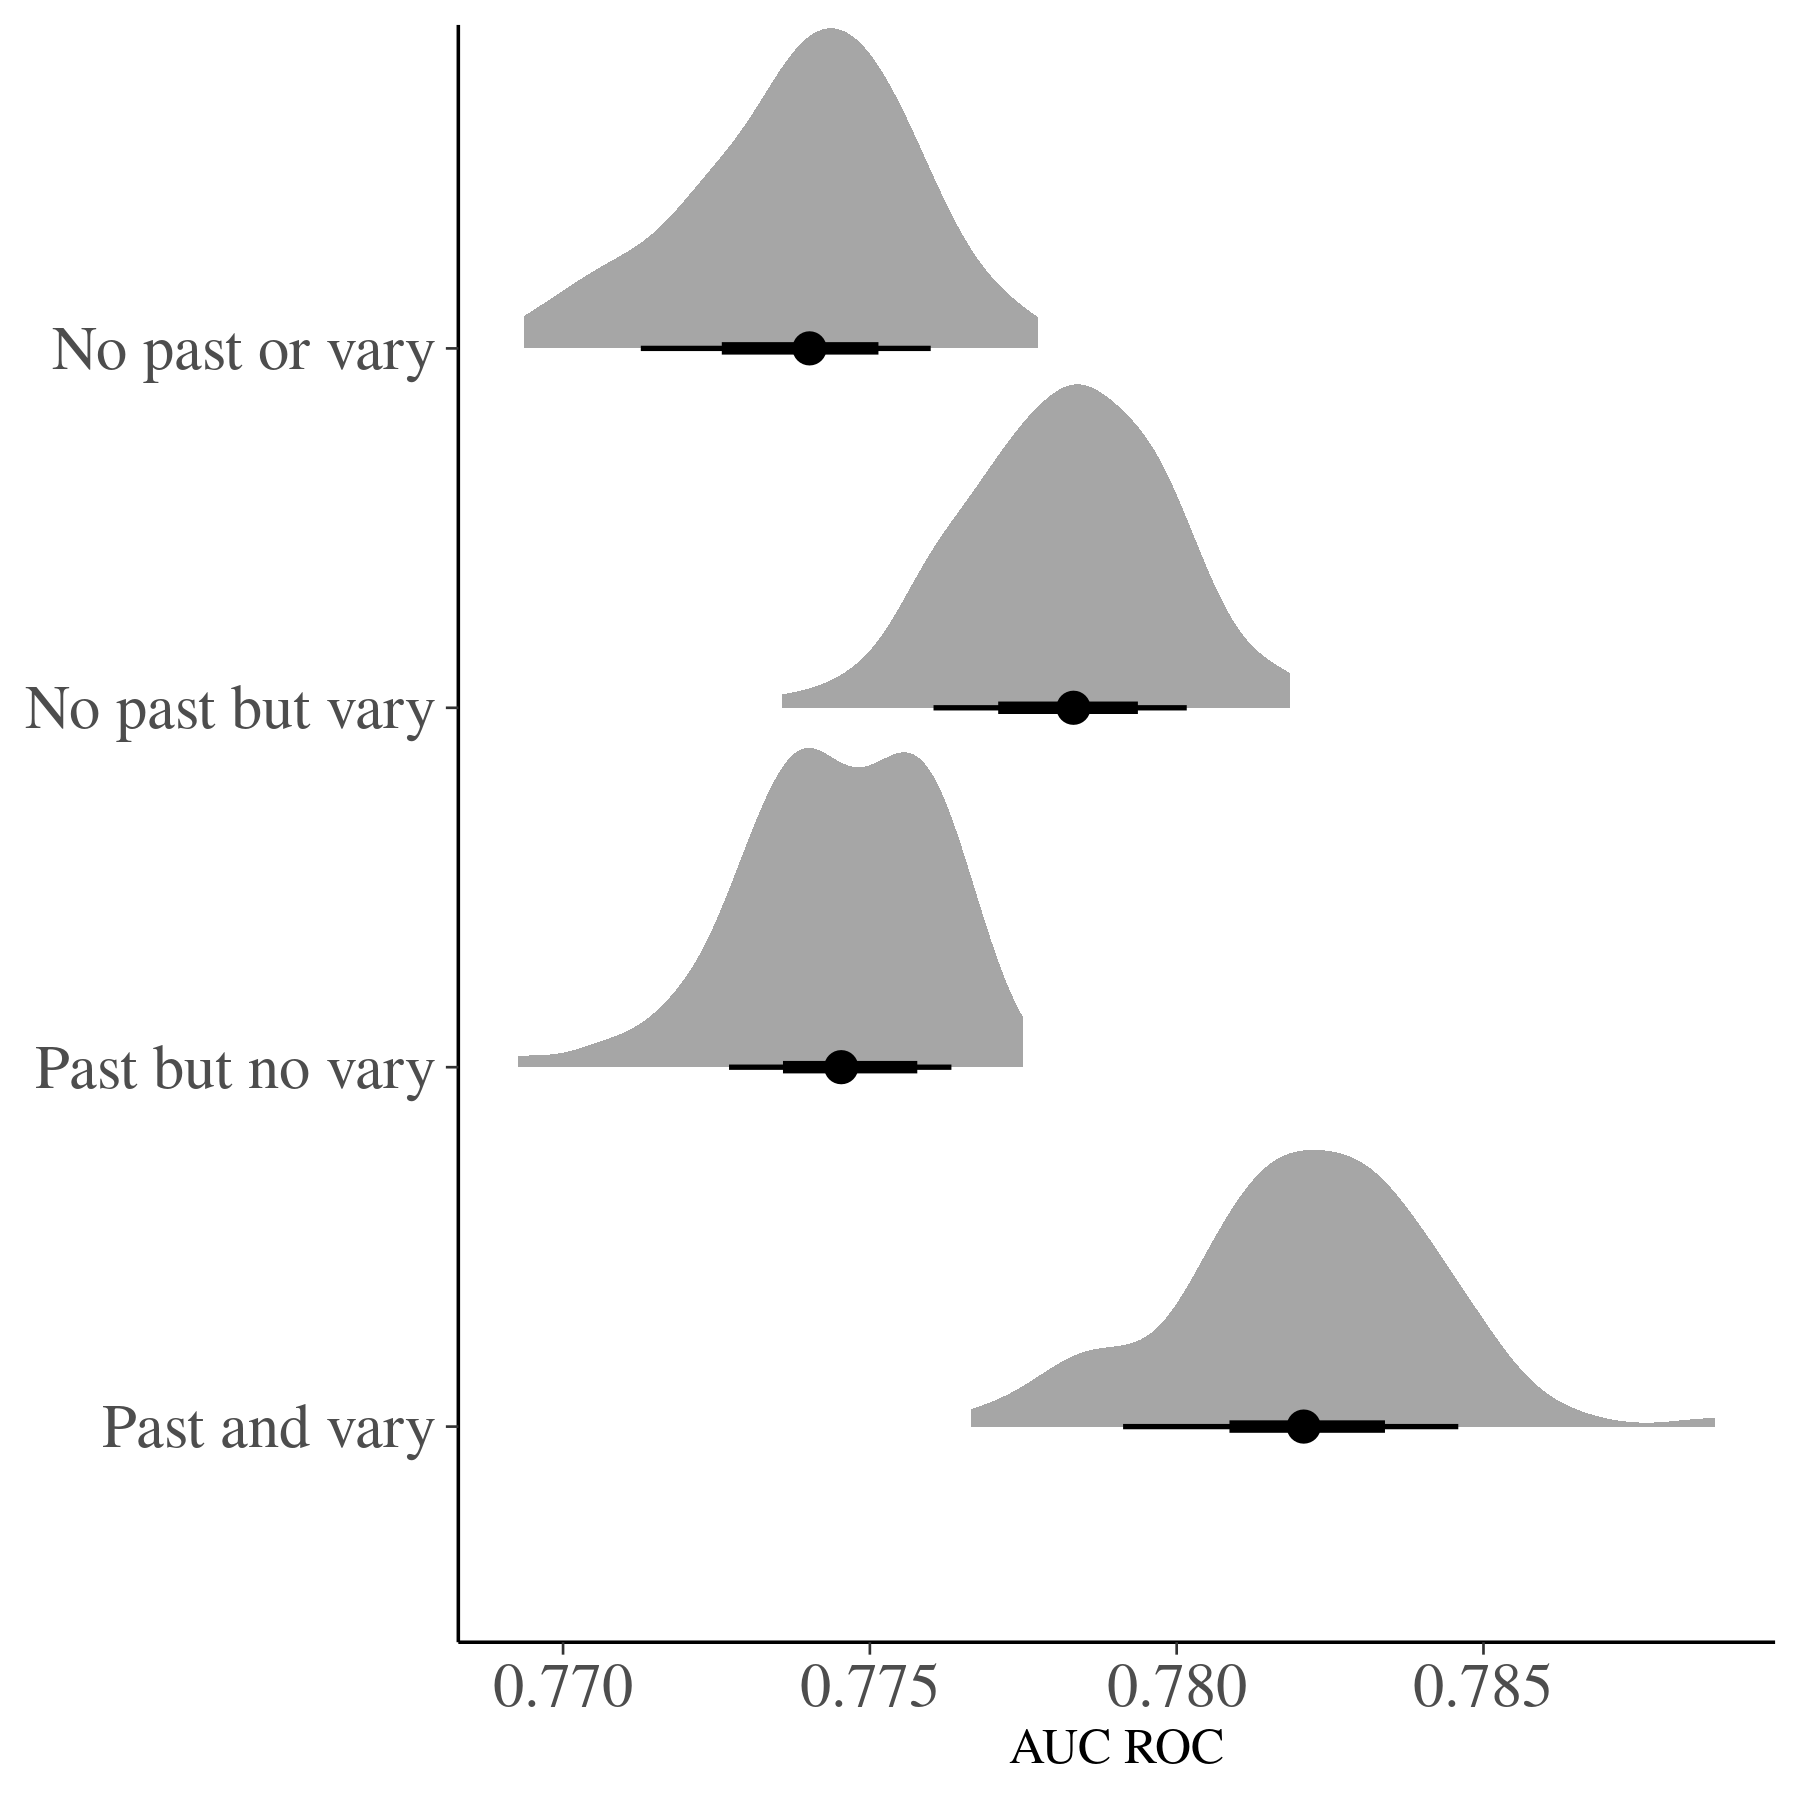
\includegraphics[width=\textwidth,height=0.5\textheight,keepaspectratio=true]{../results/figure/auc_hist_full}
  \caption{In-sample}
  \label{fig:auc_hist}
 \end{subfigure}
 \begin{subfigure}[ht]{0.45\textwidth}
  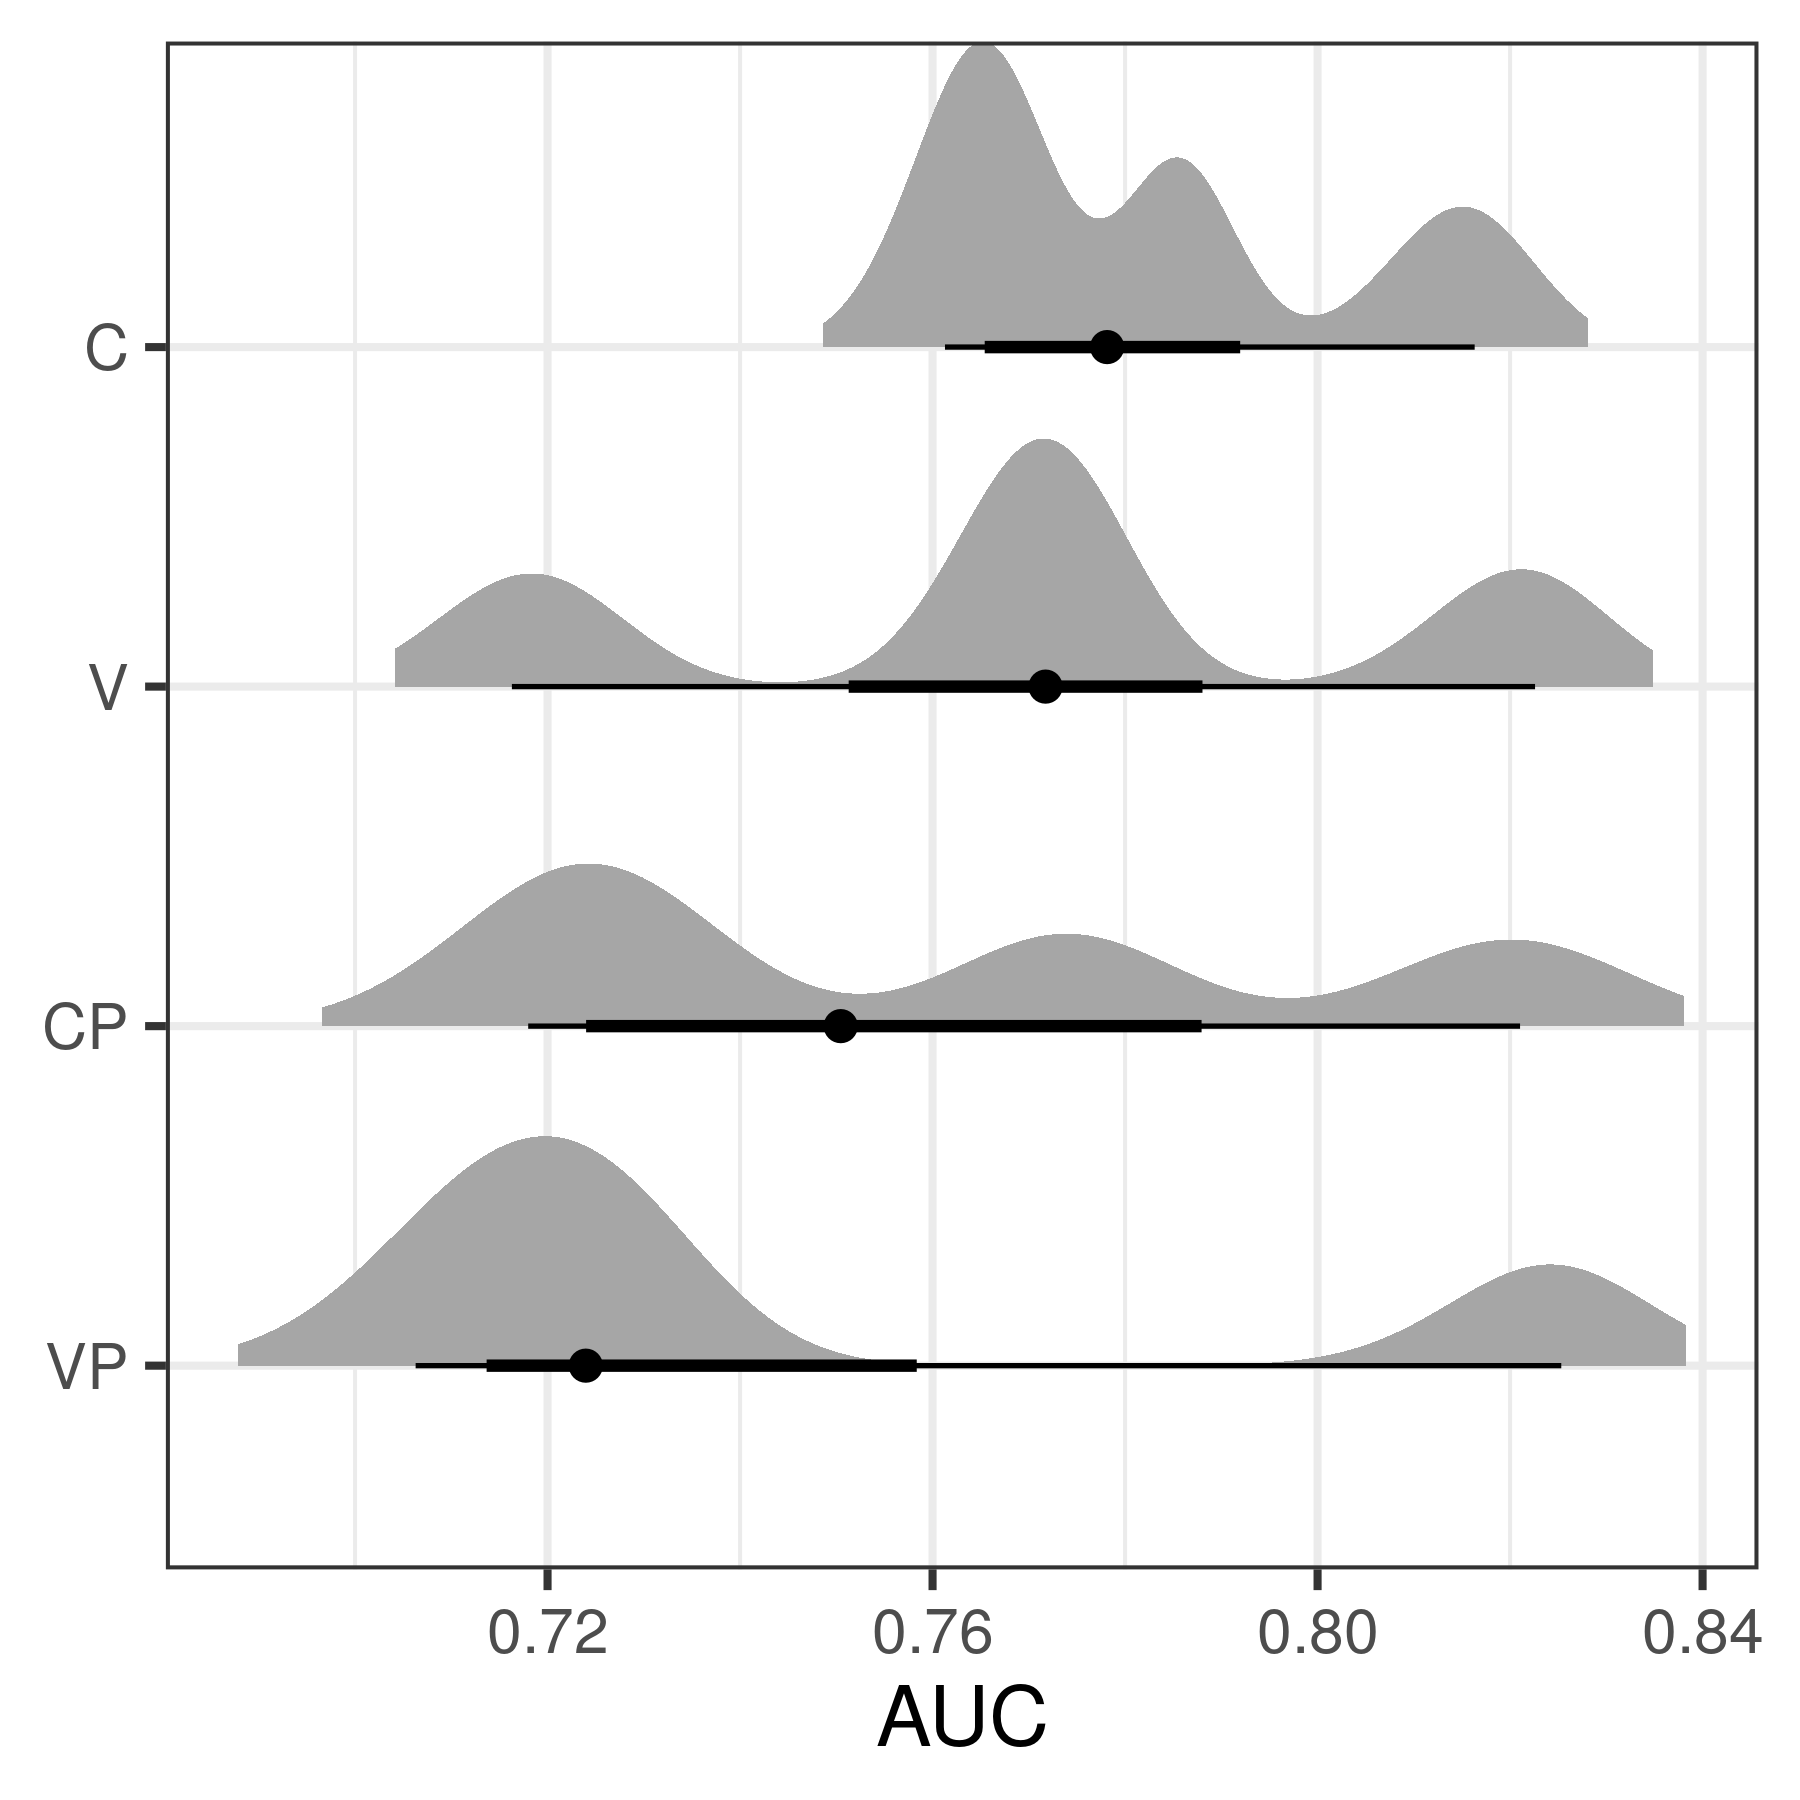
\includegraphics[width=\textwidth,height=0.5\textheight,keepaspectratio=true]{../results/figure/fold_auc_full}
  \caption{Out-of-sample}
  \label{fig:fold_auc}
 \end{subfigure}
 \caption{In-sample (\ref{fig:auc_hist}) and out-of-sample (\ref{fig:fold_auc}) AUC estimates for each of our four models. These estimates are calculated from the models posterior predictive distribution or from predictions made to new data, respectively. Models with a higher AUC values indicate better performance over models with lower AUC values. AUC is bounded between 0.5 and 1. See Table \ref{tab:model_def} for a description of each of the four models.}
 \label{fig:auc_compare}
\end{figure}

\subsection{In-sample forecasting adequacy}

The in-sample model comparisons are useful for comparing the relative ability of our models to represent the data they were fit to. Comparison between the posterior distributions of in-sample AUC for each of the four models demonstrates that all of our models have approximately equal in-sample forecasting performance (Fig. \ref{fig:auc_hist}). The parameter rich model VP has the greatest median in-sample AUC when compared to the other three models, but there is substantial overlap in their posterior distributions. Additionally, while our parameter rich model VP is possibly the most adequately performing model, the difference or improvement to performance is minimal at best -- all four models have approximately equal in-sample AUC posterior distributions. All the in-sample AUC estimates from our models are concentrated on an AUC value of 0.77. It is therefore hard to conclude that there is one ``best'' model which we can rely upon as they are all nearly functional equivalent. 

%When the posterior predictive distributions of the in-sample AUC estimates are presented over time, the similarity in adequacy between the models becomes more apparent (Fig. \ref{fig:auc_ts}). There are few major or obvious differences in model adequacy between the four models.
%% ROC model comparison time series
%\begin{figure}[ht]
% \centering
% 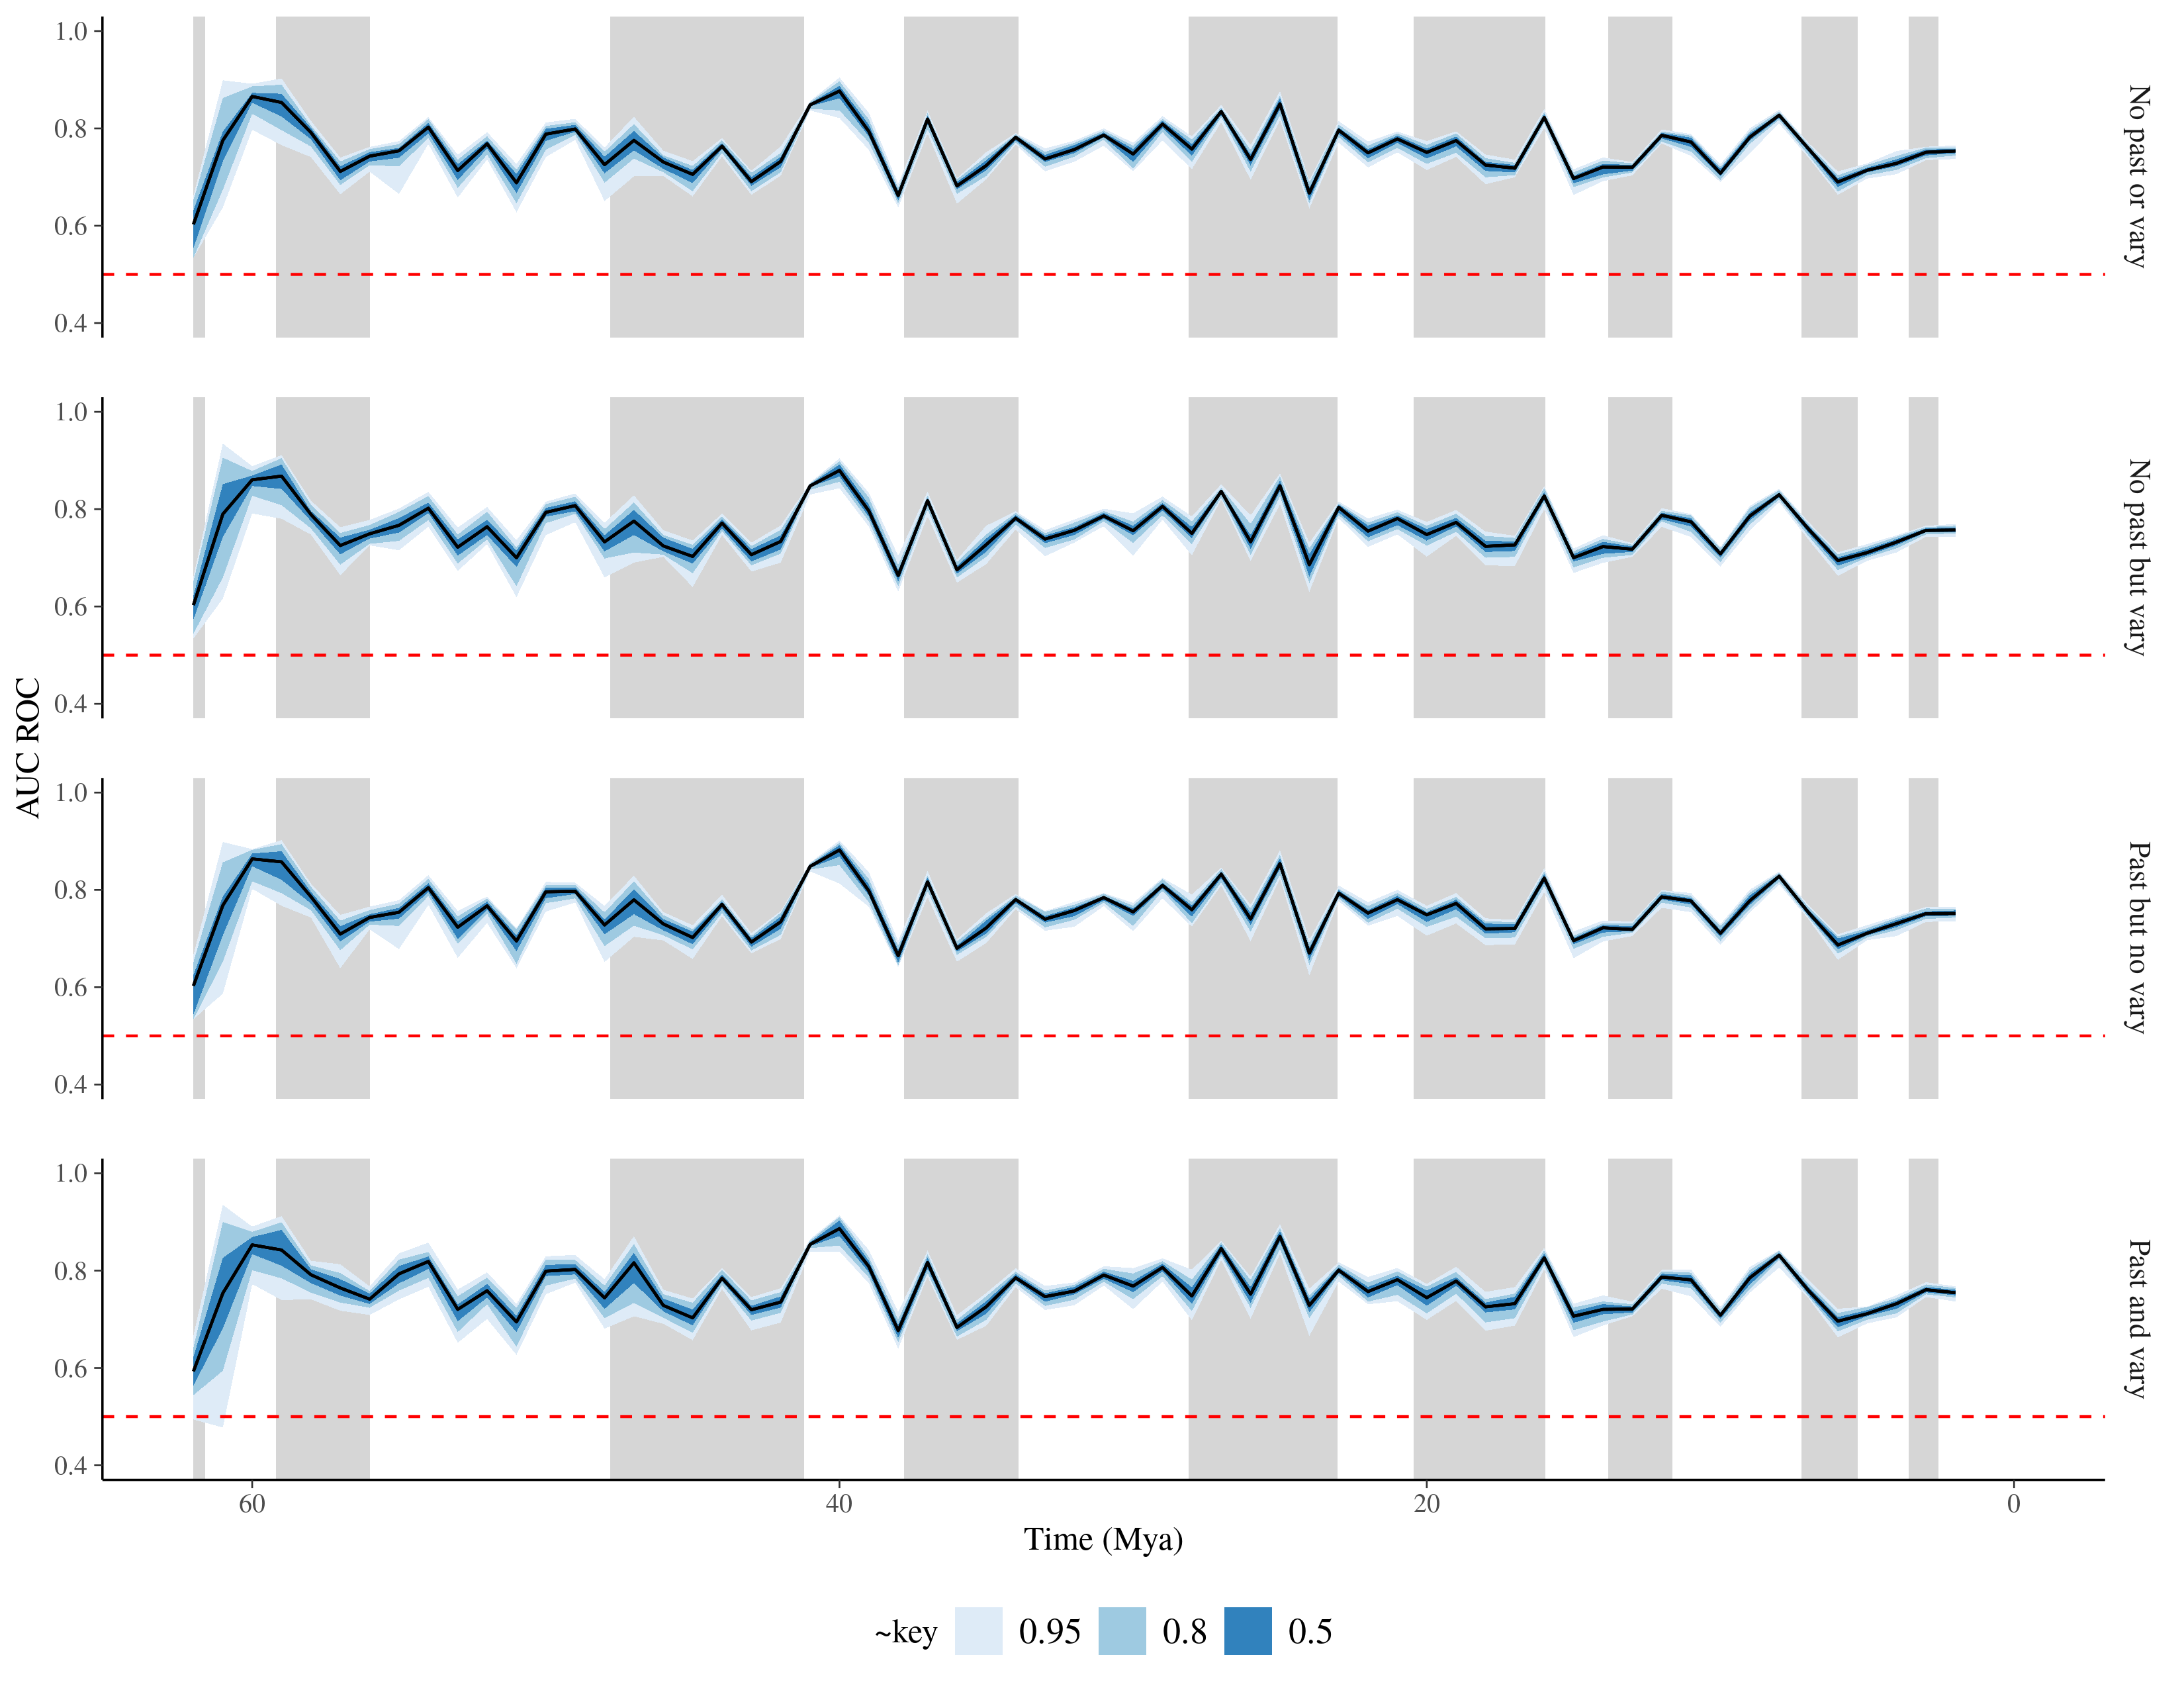
\includegraphics[width=\textwidth,height=0.5\textheight,keepaspectratio=true]{../results/figure/auc_ts_full}
% \caption{Comparison between the posterior predictive AUC estimates for each of the time intervals for each of the four models. These estimates are reflections of each model's fit to the various time intervals. The red line corresponds to the median AUC value, while the envelopes correspond to multiple credible intervals as indicated in the legend. In all cases, higher AUC values indicate greater predictive performance versus lower AUC values.}
% \label{fig:auc_ts}
%\end{figure}


%When the posterior predictive distributions of the in-sample AUC estimates are presented by taxonomic group, some heterogeneity in model adequacy is revealed (Fig. \ref{fig:auc_taxon}). While in all cases the model with the highest average in-sample AUC is the parameter-rich ``past and vary'' model, the amount of difference between the models varies by taxonomic group in ways not observable from the pooled estimates (Fig. \ref{fig:auc_hist}). For example, the difference between the ``past and vary'' model and the others is more pronounced for Calcareous nannoplankton and Dinoflagellates, and smaller for the Foraminifera and Radiolaria. 
%\begin{figure}[ht]
% \centering
% 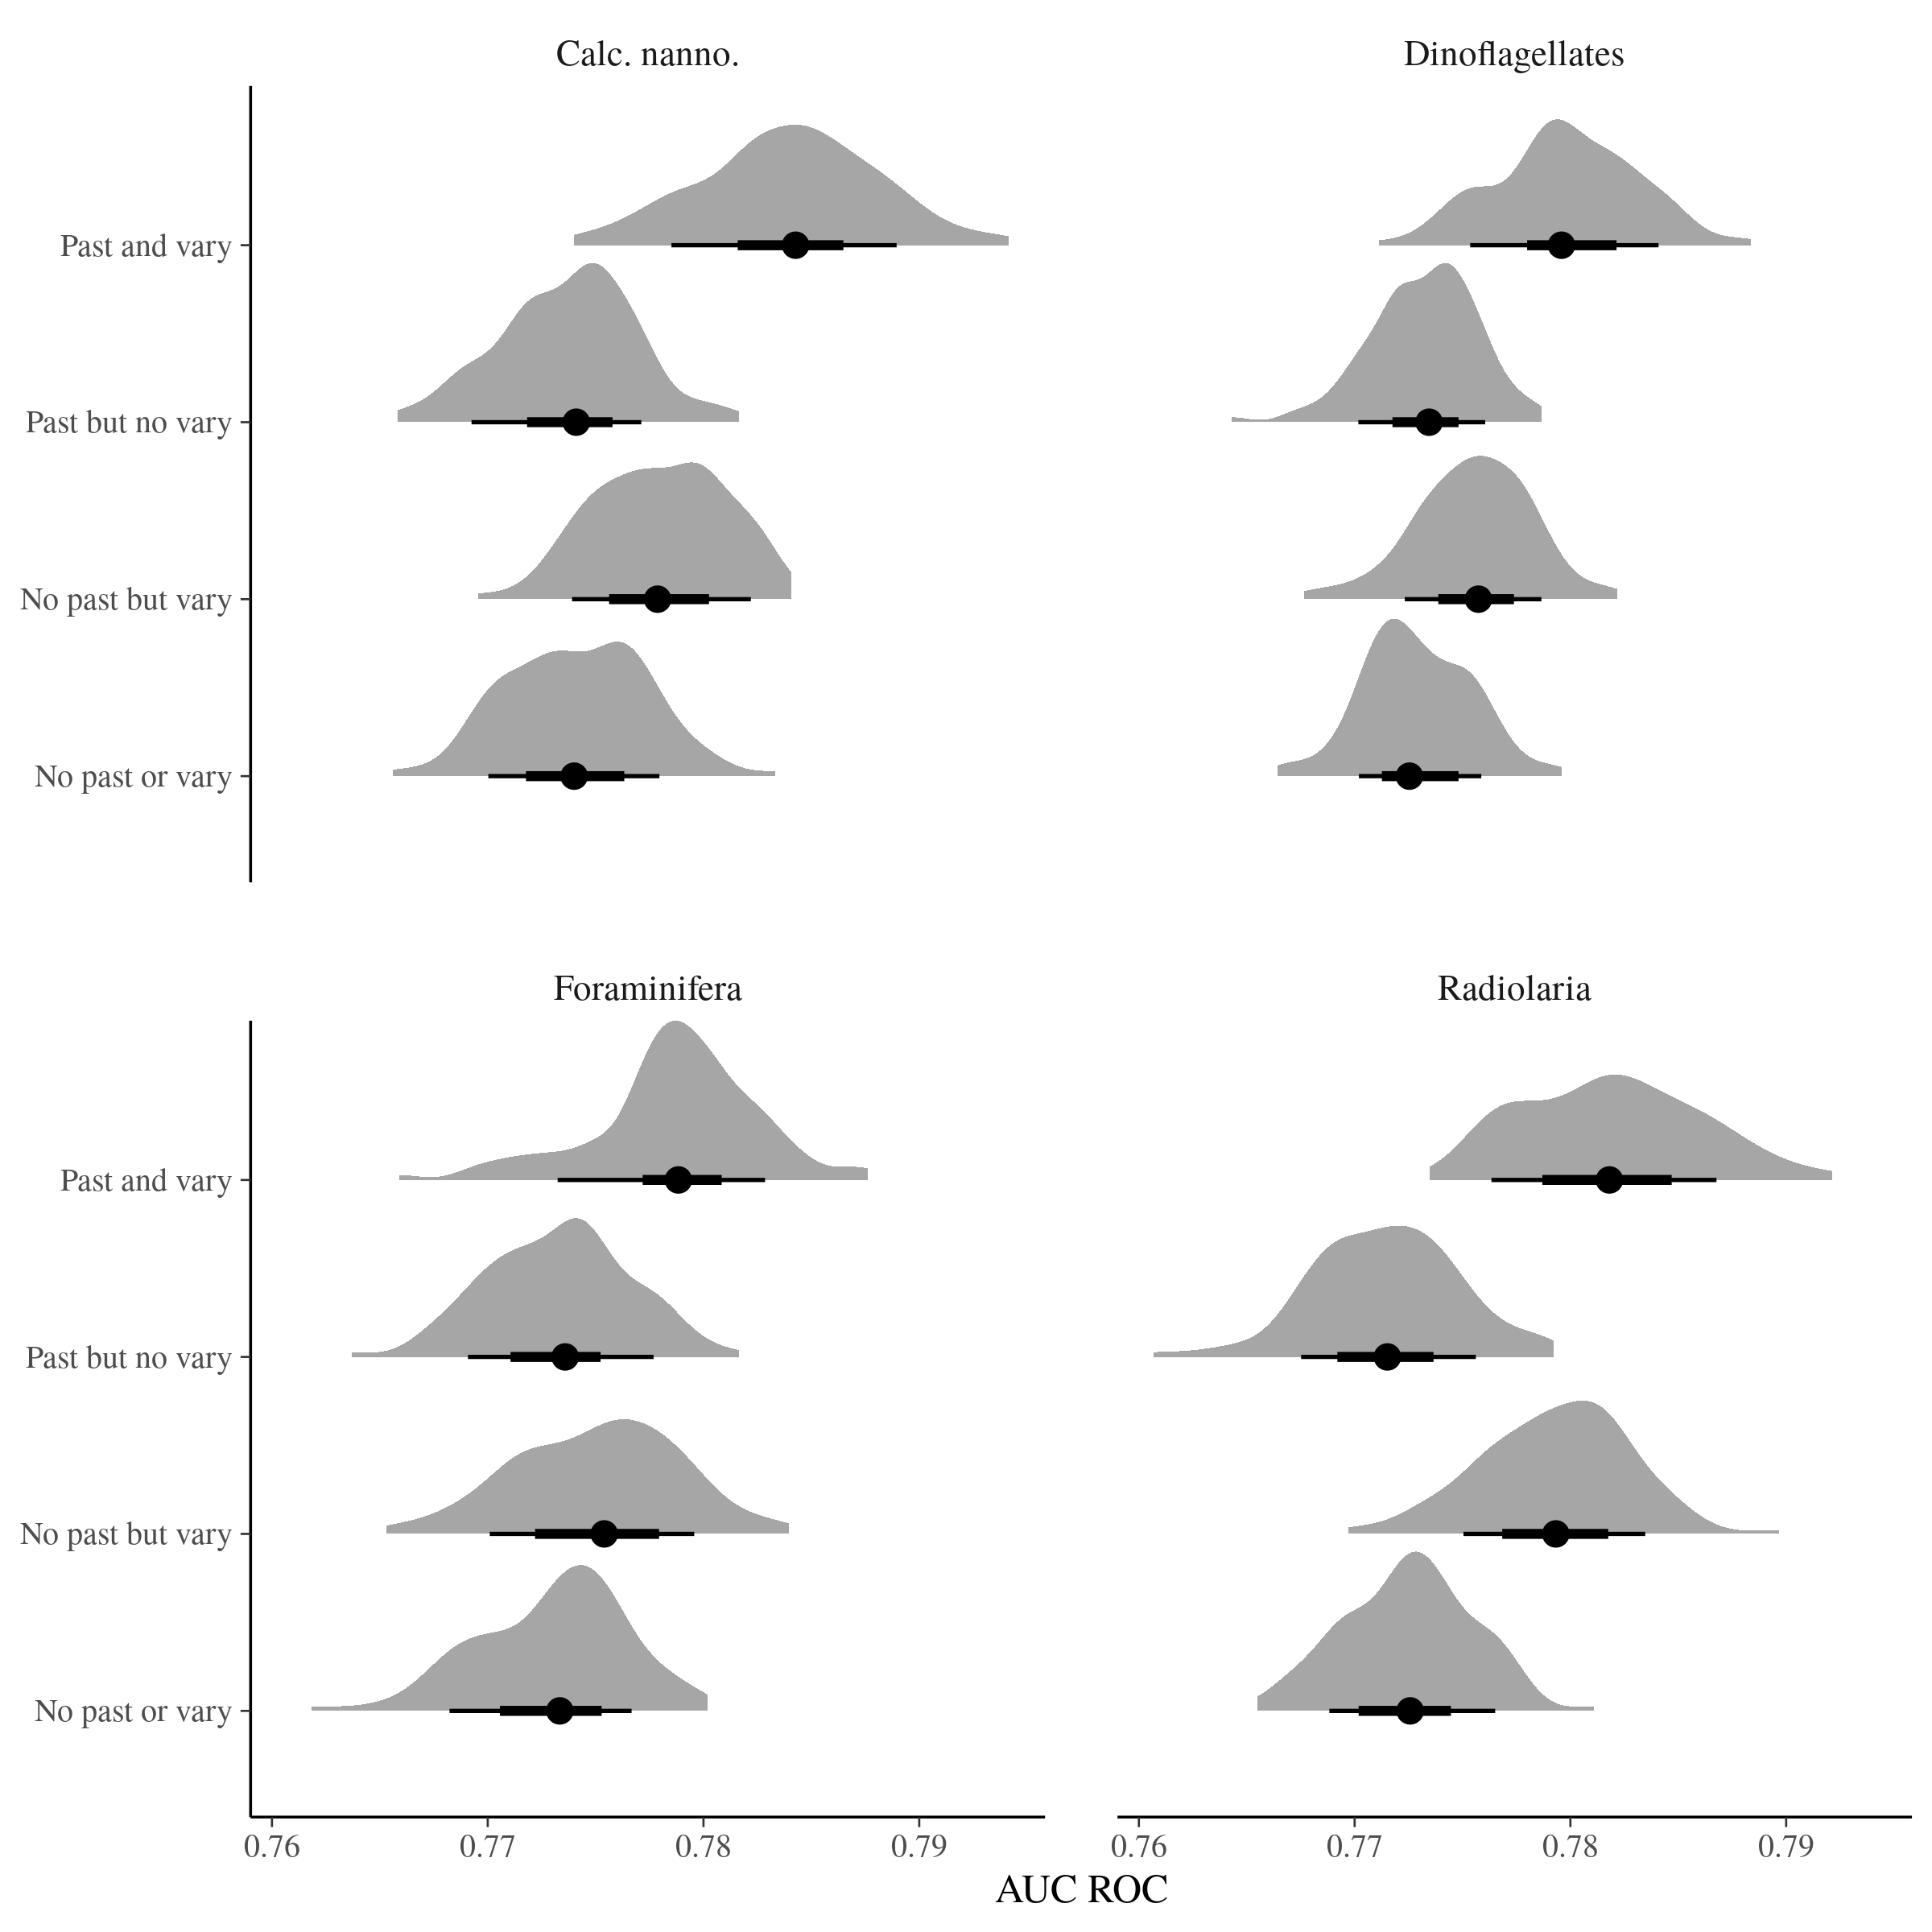
\includegraphics[width=\textwidth,height=0.5\textheight,keepaspectratio=true]{../results/figure/auc_taxon_full}
% \caption{Comparison of posterior predictive AUC estimates for each of the four models, arranged by taxonomic group. These estimates reflect each model's fit to the various taxonomic groups present in this analysis. The densities reflect the posterior distribution of the estimates, and below each density is marked the median AUC value along with the 50\% and 80\% credible intervals. In all cases, higher AUC values indicate greater predictive performance versus lower AUC values.}
% \label{fig:auc_taxon}
%\end{figure}


Depending on the taxon-model combination, there are between zero and 4 time intervals where our posterior distribution of in-sample AUC has a median value less than or equal to 0.5 (Fig. \ref{fig:auc_taxon_time}). However, this pattern is absent for the posterior estimates of in-sample AUC for Foraminfera and Radiolaria as fit by the VP model. In contrast, there are fewer periods of low model performance for calcareous nannoplankton and Dinoflagellates as estimated from our VP model than in those estimates from the other three model variations.

\begin{figure}[ht]
 \centering
 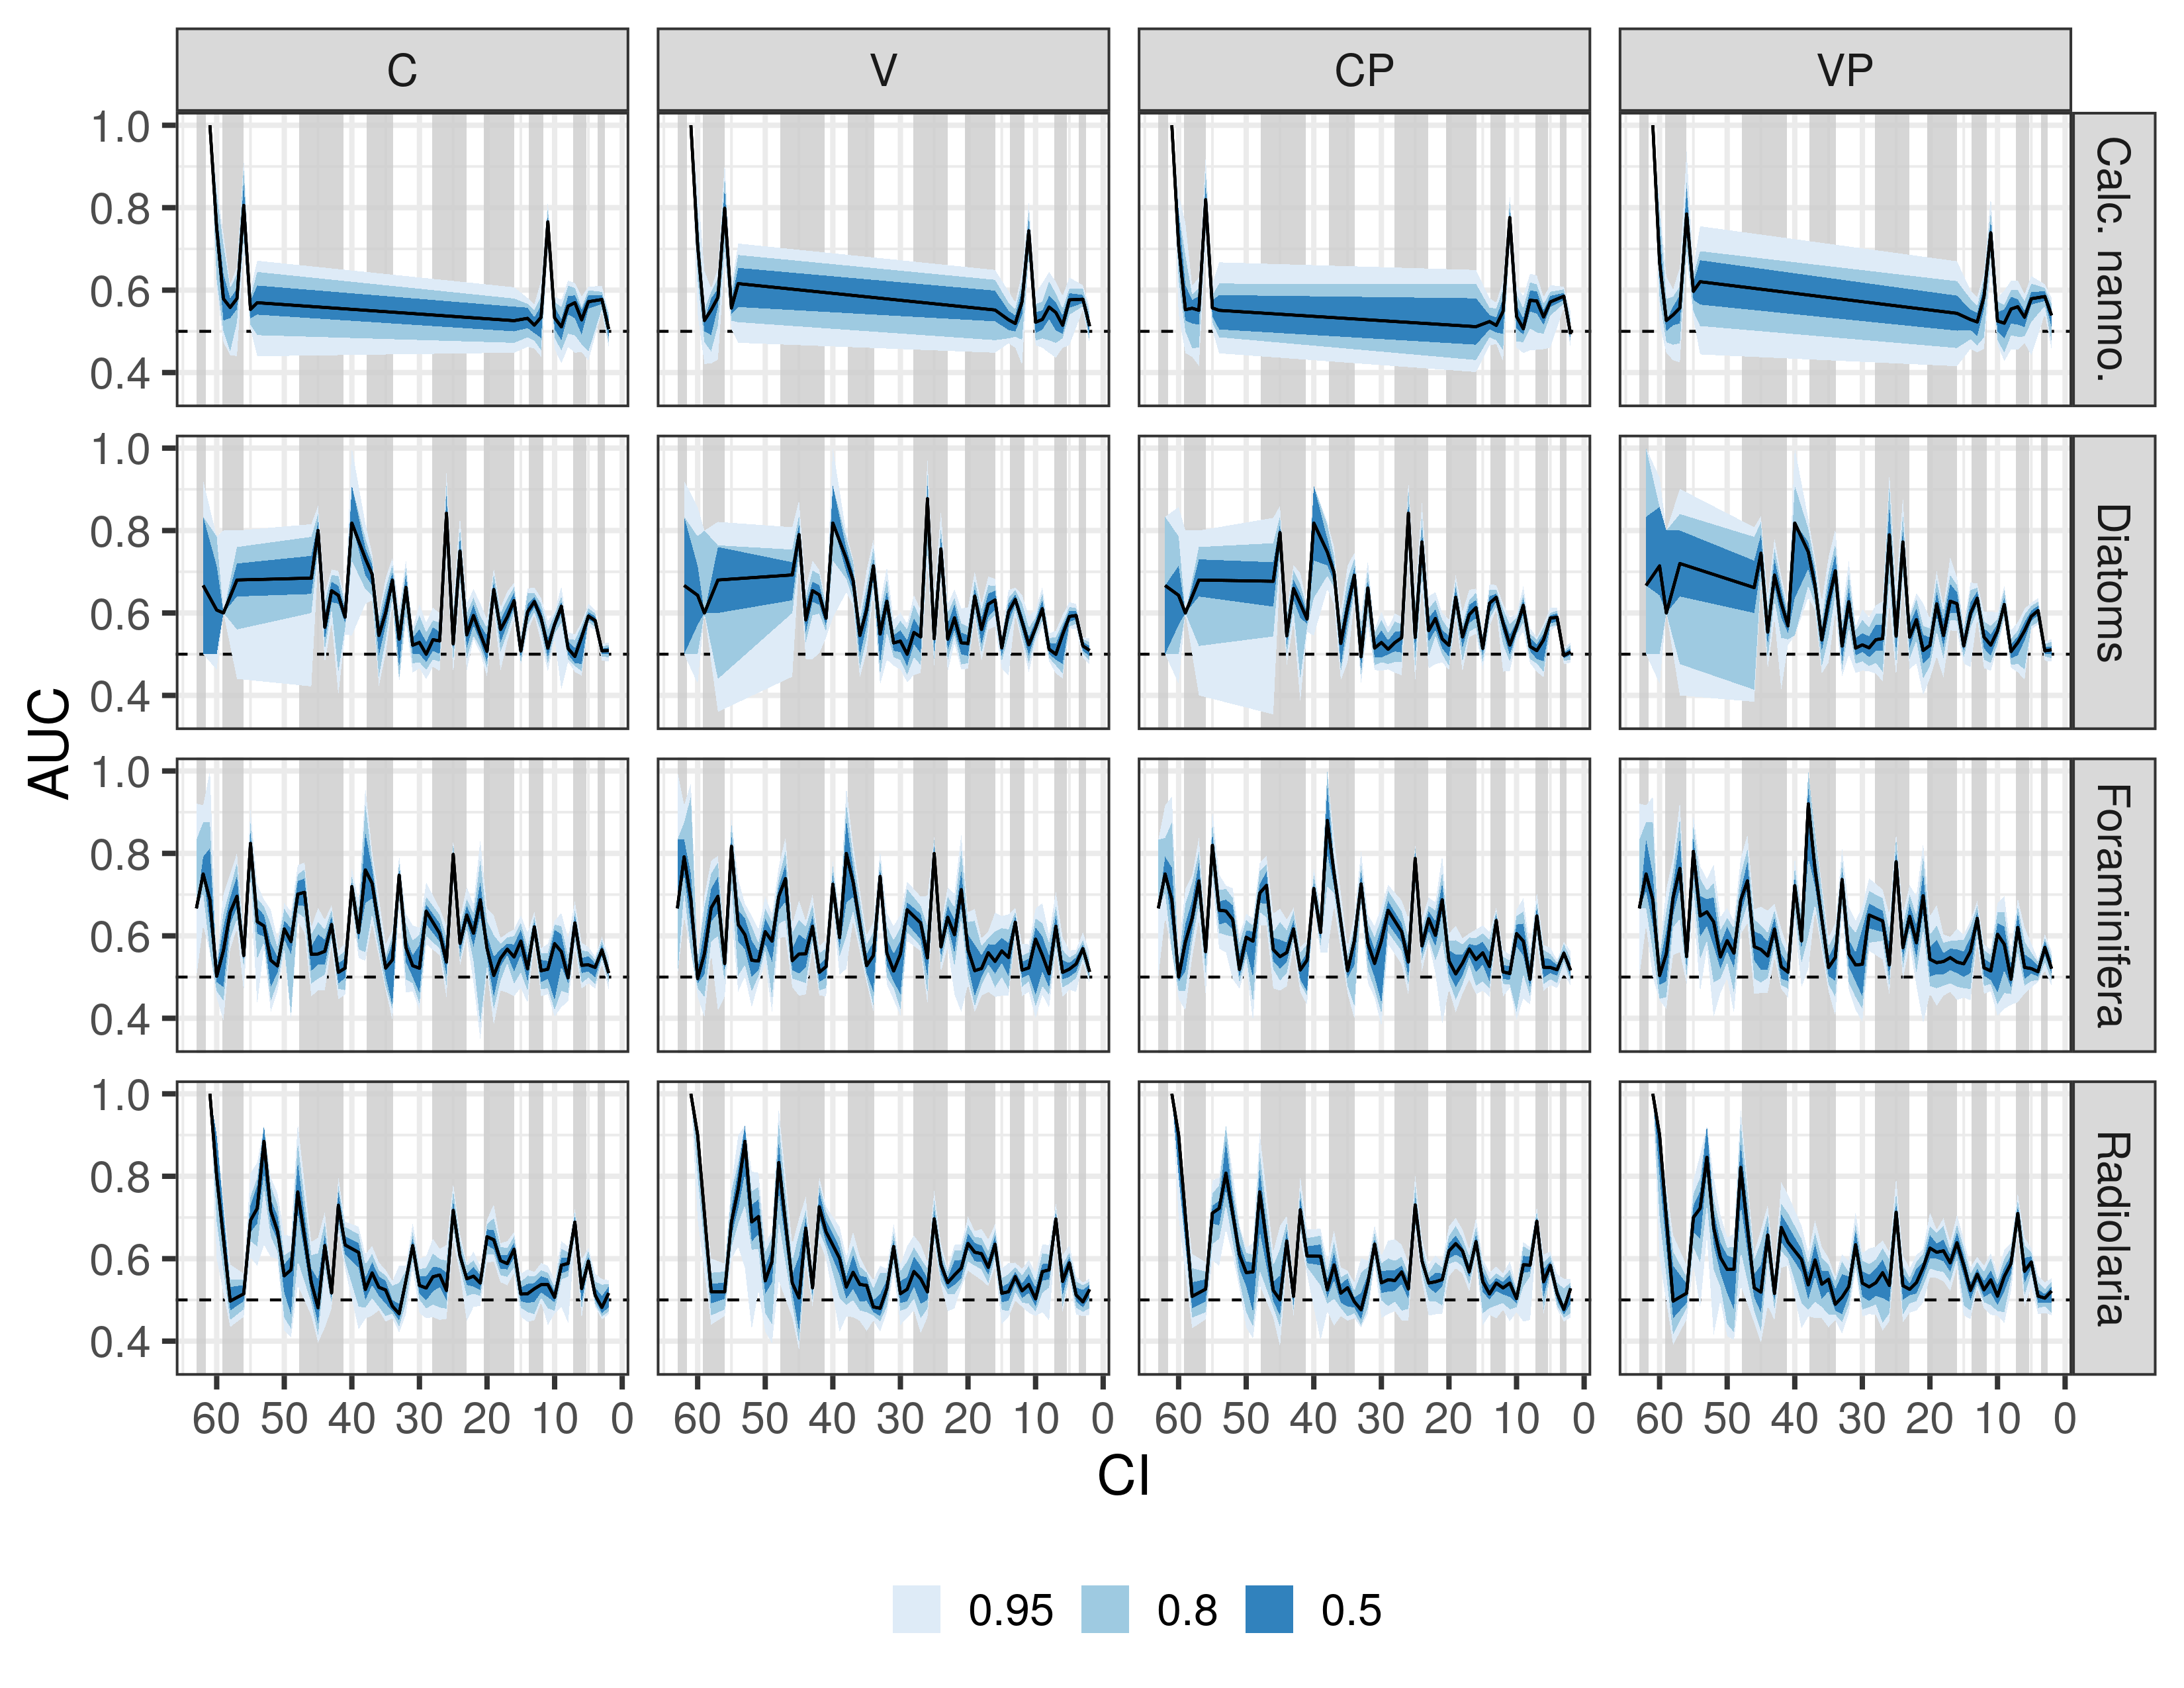
\includegraphics[width=\textwidth,height=0.5\textheight,keepaspectratio=true]{../results/figure/auc_taxon_time_full}
 \caption{Comparison of in-sample forecasting performance measured by AUC for each of the four models, arranged over time and by taxonomic group. These estimates reflect each model's fit to the various taxonomic groups over time. The black line corresponds to the median AUC value, while the envelopes correspond to multiple credible intervals as indicated in the legend. In all cases, higher AUC values indicate greater predictive performance versus lower AUC values. See Table \ref{tab:model_def} for a description of each of the four models.}
 \label{fig:auc_taxon_time}
\end{figure}




\subsection{Out-of-sample forecasting performance}

Expected out-of-sample forecasting performance was estimated using five-fold cross-validation for time series \citep{Arlot2010,Bergmeir2016}. The resulting distribution when all folds are combined is highly multimodal as expected given that they are fit to and estimated from different data sets with different numbers of observations \citep{ESL}. This multimodality increases with model complexity (Fig. \ref{fig:fold_auc}), most likely because the complex models allow for predictor effects to vary with time, allowing a greater range in possible parameter values which in turn yield a greater range of posterior predictions.

Comparison the in-sample AUC estimates to the expected out-of-sample AUC estimates reveals a similar range in performance for all models (Fig. \ref{fig:auc_hist}, \ref{fig:fold_auc}). Interestingly, the differences in posterior predictive distributions of AUC between the four model variations is reduced in out-of-sample prediction. For example, the VP model no longer has the greatest median AUC of the four models (Fig. \ref{fig:fold_auc}). For this reason the rank order of median out-of-sample AUC is different from the rank order of median in-sample AUC. However, making interpretations based only on the median AUC estimates is incorrect -- our estimates are the full posterior, not individual points. Because of this, the four models are effectively indistinguishable in their out-of-sample forecast performance (Fig. \ref{fig:fold_auc}).

%A slight decrease in performance when dealing with out-of-sample observations makes sense: each of the models fit during cross-validation is based on fewer data than the model fit on the full data (between 1/5th to 4/5ths of the original). Additionally, a potential decrease in precision when forecasting the future of extinction risk is almost to be expected as the future is not necessarily the same as the past. However, the similarly between the in-sample and out-of-sample results indicates that our model is fairly robust to how extinction intensity has changed over the Cenozoic. 

%This result means that we would expect to correctly rank two species in order of most to least likely to go extinct 70-80\% of the time. However, this expected out-of-sample performance is approximately the same as the in-sample performance results (Fig. \ref{fig:auc_hist}), indicating that our models would yield consistent results when generalized to future extinctions.

%When the posterior predictive distribution of expected out-of-sample AUC is presented as a time series, the similarity between the models is even more apparent (Fig. \ref{fig:fold_auc_time}). While the width of the credible intervals at various time points varies between the models, the overall picture of expected out-of-sample AUC is almost identical when you compare the models -- periods of relatively better or worse performance map identically between the time series.
%\begin{figure}[ht]
% \centering
% 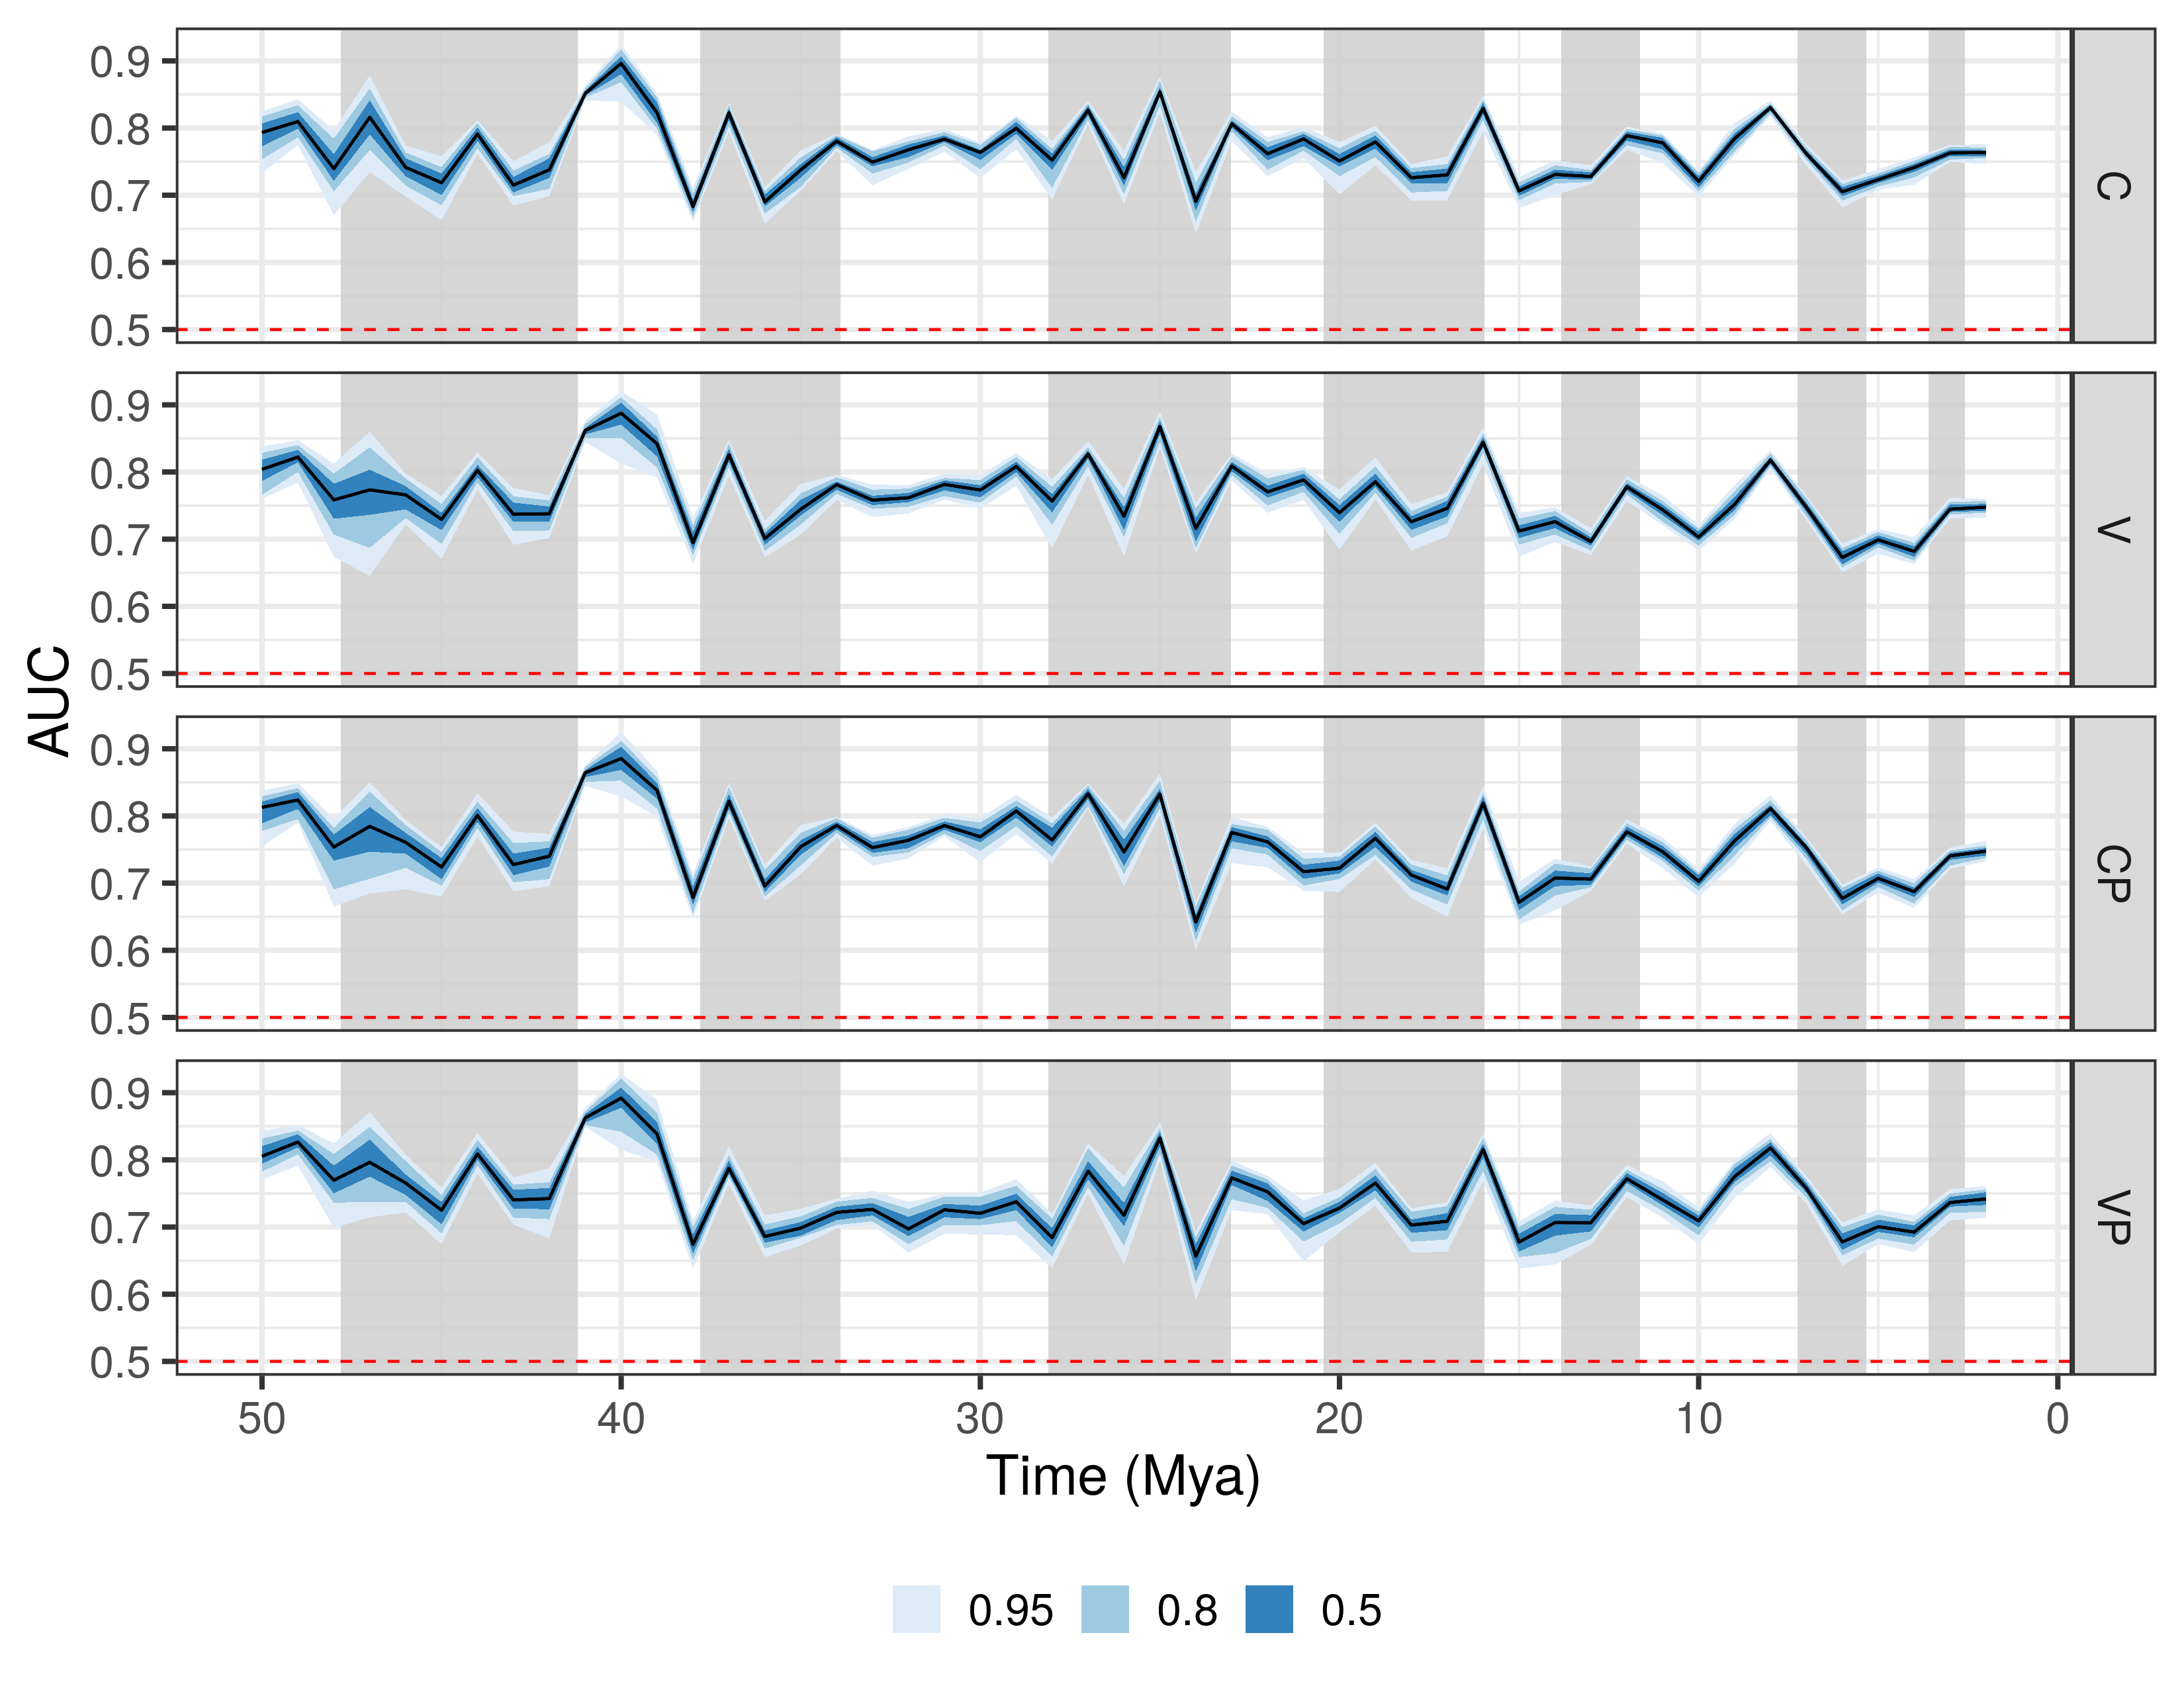
\includegraphics[width=\textwidth,height=0.5\textheight,keepaspectratio=true]{../results/figure/fold_auc_time_full}
% \caption{Comparison of out-of-sample AUC values calculated for each of the million year intervals for each of the four models. The AUC of the individual My intervals within each fold is plotted to highlight the heterogeneity in performance within and between folds. This presentation decomposes each of the 12-million year folds (Fig. \ref{fig:fold_auc}) into the predictions made for each of the million-year intervals. The red line corresponds to the median AUC estimate, with the envelopes corresponding to multiple credible intervals as indicated in the legend.}
% \label{fig:fold_auc_time}
%\end{figure}
%We can also compare expected out-of-sample AUC by taxonomic group for each of the models (Fig. \ref{fig:fold_auc_taxon}). These comparisons reveal a lot about the differences in predictive potential of the taxonomic groups. For example, the posterior predictive distributions of out-of-sample AUC for Foraminifera from all four models are approximately identical. In contrast, expected out-of-sample AUC for Radiolaria exhibits the same or similar pattern in relative model performance to the pooled comparisons (Fig. \ref{fig:fold_auc}). Additionally, we can state that our out-of-sample predictions for calcareous nannoplankton and dinoflagellates are not necessarily as precise as our estimates for Foraminifera or even Radiolaria. These results indicate that out-of-sample predictions may be easier for some taxonomic groups than others (e.g. Foraminifera versus Dinoflagellates.
%\begin{figure}[ht]
% \centering
% 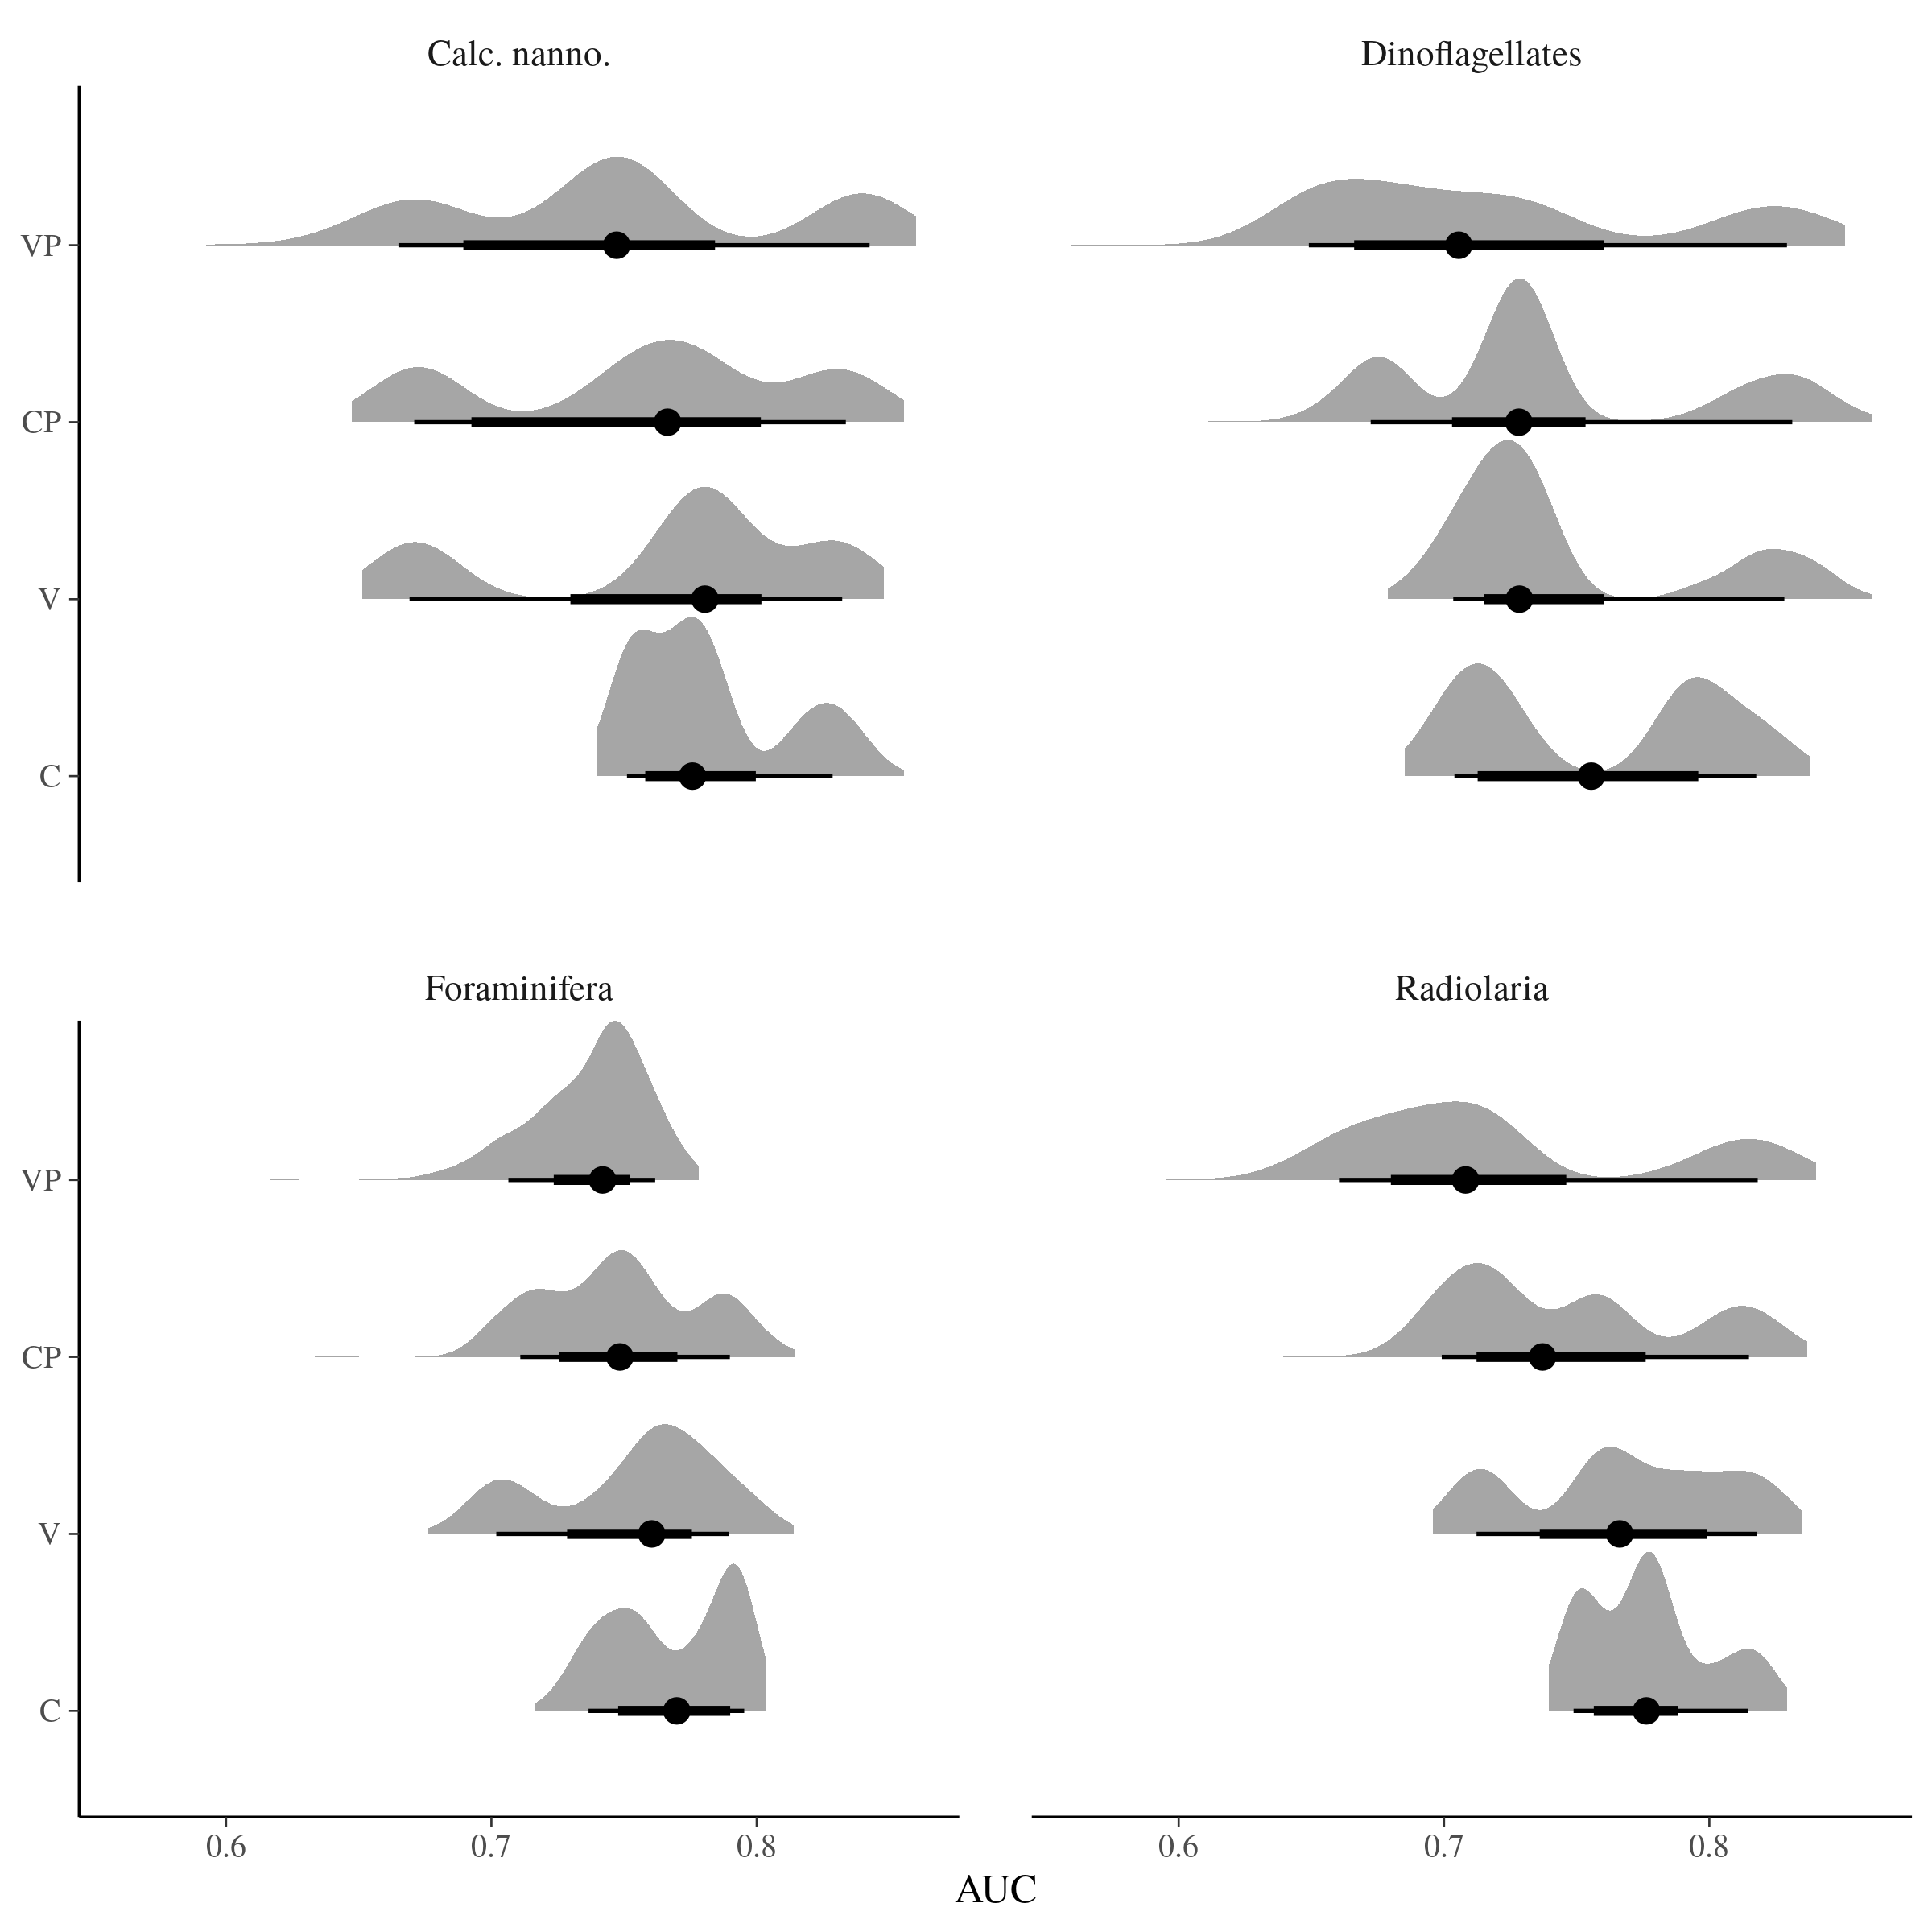
\includegraphics[width=\textwidth,height=0.5\textheight,keepaspectratio=true]{../results/figure/fold_auc_taxon_full}
% \caption{Comparison of out-of-sample AUC values aggregated by taxonomic group for each of the four models. Depicted for each taxon-model combination is an aggregate density of all posterior predictive estimates for each of four folds -- cross-validation estimates are commonly multi-modal as each fold presents its own challenges for prediction. Beneath these densities is marked the median estimate along with 50\% and 80\% credible intervals.}
% \label{fig:fold_auc_taxon}
%\end{figure}
%

The posterior predictive distribution of expected out-of-sample AUC over time and across taxonomic groups are nearly identical for each of the four models (Fig. \ref{fig:fold_auc_taxon_time}). 

In the analysis of the in-sample forecast performance of the four models, we noted that there were time intervals where our predictions were no better than random (Fig. \ref{fig:auc_taxon_time}). This occurrence is generally much rarer for the posterior distribution of AUC from the out-of-sample forecasts. The major exception to this pattern are our estimates for the Dinoflagellates, which have at least one time interval for all four models in which the median AUC of the out-of-sample forecasts were no better random. The only other group for which median posterior predictive estimate of out-of-sample AUC reaches 0.5 is calcareous nannoplankton, and then only with the V model.
\begin{figure}[ht]
 \centering
 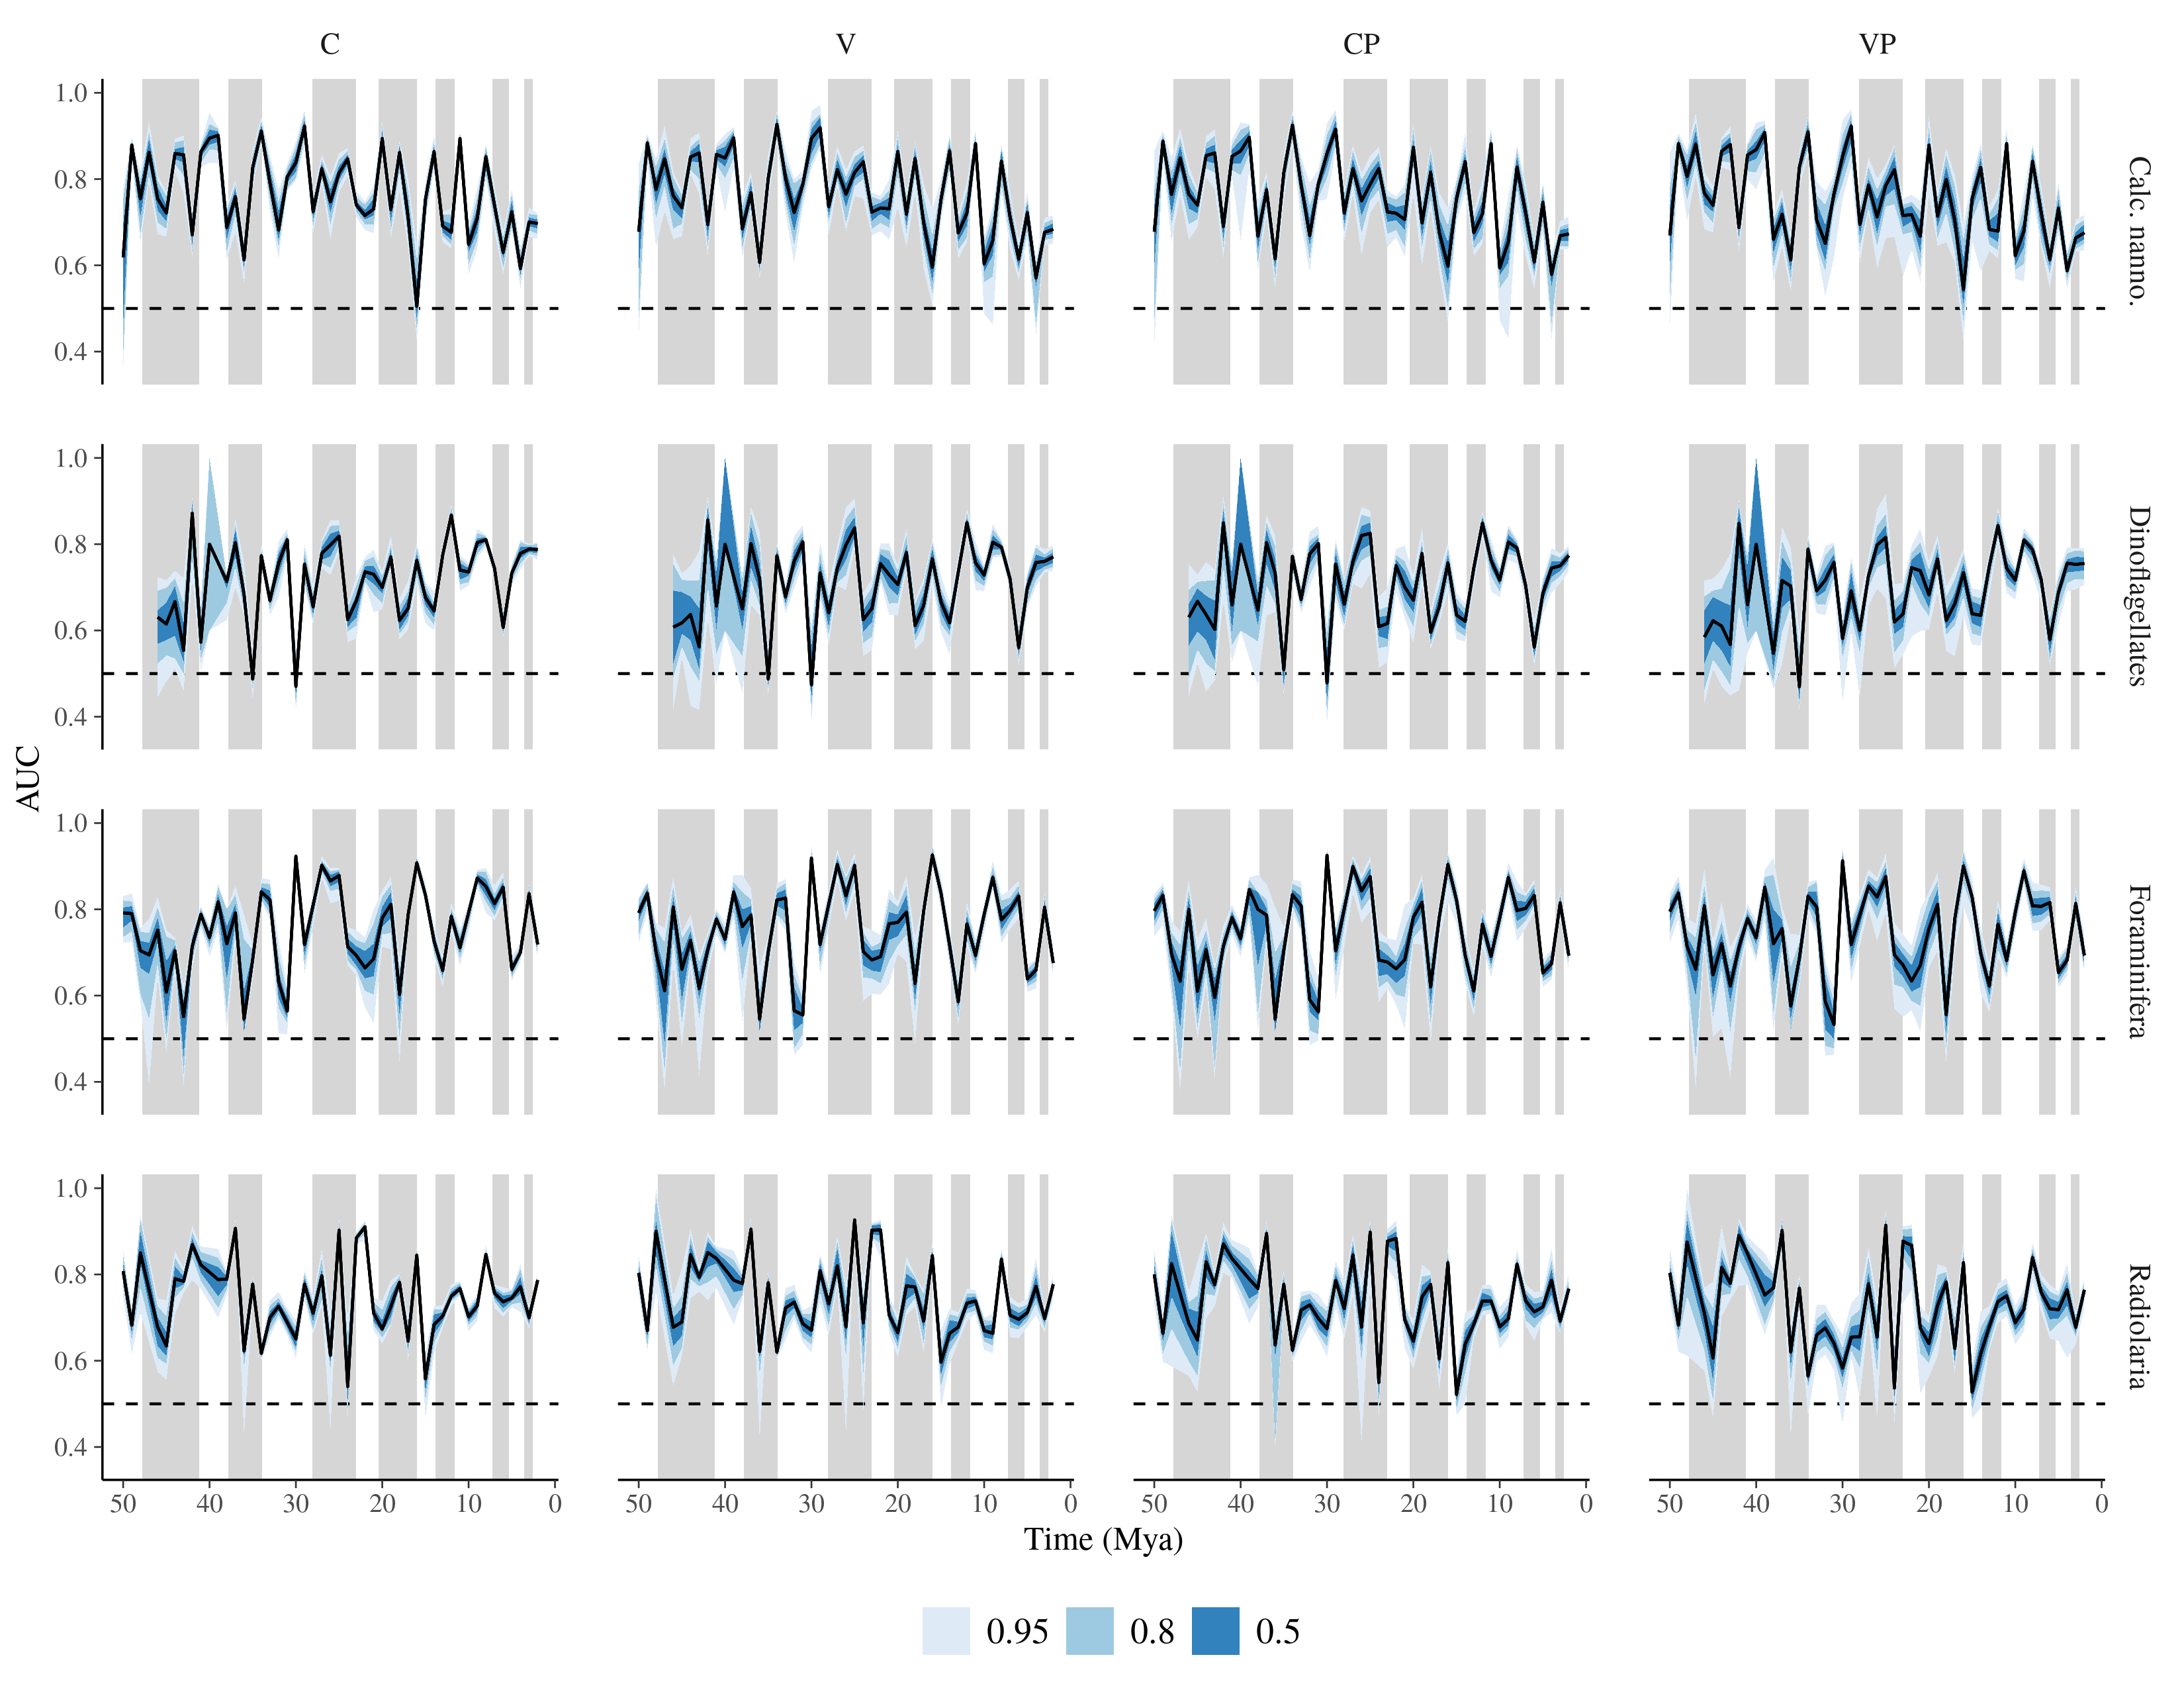
\includegraphics[width=\textwidth,height=0.5\textheight,keepaspectratio=true]{../results/figure/fold_auc_taxon_time_full}
 \caption{Comparison of out-of-sample AUC values over time as aggregated by taxonomic group for each of the four models. The AUC of the individual My intervals within each fold is plotted to highlight the heterogeneity in performance within and between folds. This presentation decomposes each of the 12-million year folds by each of the taxonomic groups into the predictions made for each of the million-year intervals. The black line corresponds to the median AUC estimate, with the envelopes corresponding to multiple credible intervals as indicated in the legend. See Table \ref{tab:model_def} for a description of each of the four models.}
 \label{fig:fold_auc_taxon_time}
\end{figure}


We compared the difference in our AUC estimates from the out-of-sample forecasts to the AUC estimates from our in-sample forecasts by subtracting the in-sample AUC estimates from the out-of-sample AUC estimates (Fig. \ref{fig:oos_ins_diff}). A difference in AUC close to 0 indicates complete congruence between the in-sample and out-of-sample forecasts. A positive difference indicates that our out-of-sample forecasts are actually higher performing than our in-sample forecasts, while negative difference indicates poorer out-of-sample performance than in-sample forecast. Divergences between our out-of-sample and in-sample forecasts are rare and tend to not form multimillion year patters, consistent with the broad visual congruence between the in-sample and out-of-sample forecast performance (Fig. \ref{fig:auc_taxon_time}, \ref{fig:fold_auc_taxon_time}). The only major multimillion year pattern indicating significantly poorer out-of-sample forecast performance than in-sample forecast performance is for Radiolaria based on the VP model concentrated around 30 Mya (Fig. \ref{fig:oos_ins_diff}).

\begin{figure}[ht]
 \centering
 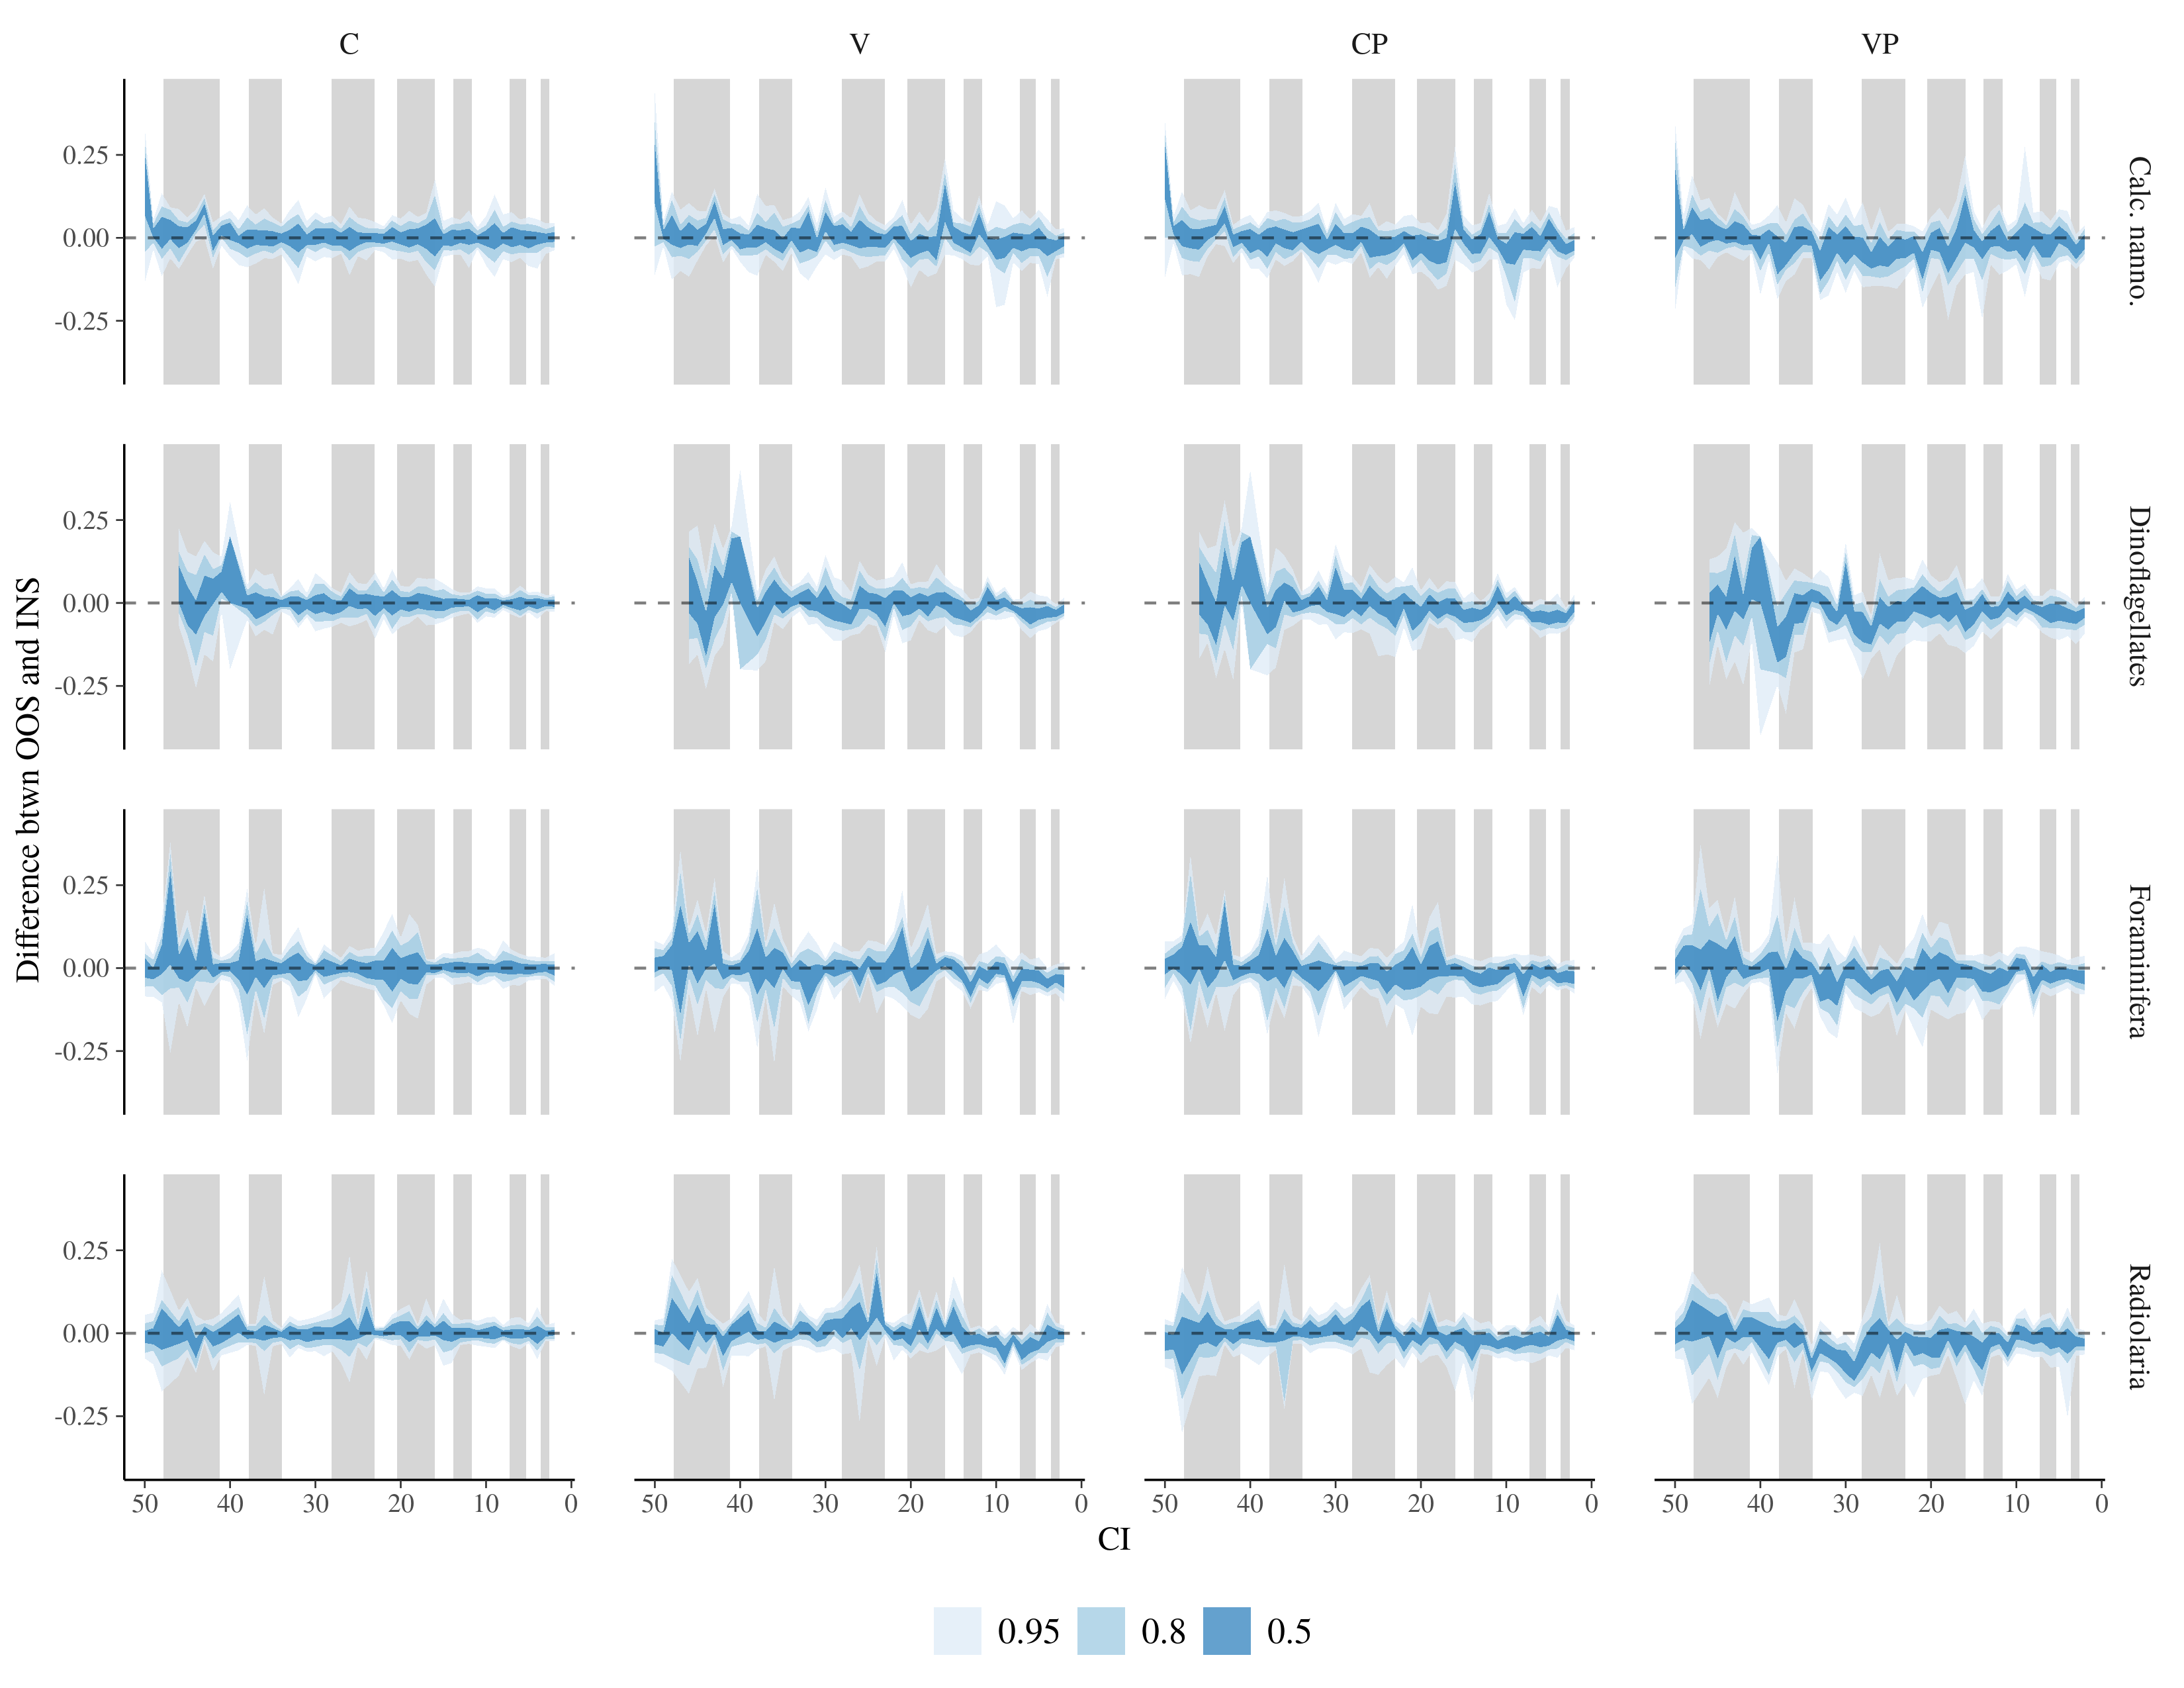
\includegraphics[width=\textwidth,height=0.5\textheight,keepaspectratio=true]{../results/figure/auc_diff}
 \caption{Comparison between our out-of-sample forecasts and in-sample forecasts for all models. This value is calculated as the values presented in Figure \ref{fig:fold_auc_taxon_time} minus those values presented in Figure \ref{fig:auc_taxon_time}. A differences close to 0 indicate complete congruence between in-sample and out-of-sample forecasts, while a positive difference indicates that our out-of-sample forecasts are actually higher performing than our in-sample forecasts, and a negative difference indicates poorer out-of-sample performance than in-sample forecast. See Table \ref{tab:model_def} for a description of each of the four models.}
 \label{fig:oos_ins_diff}
\end{figure}



%Looking at four randomly sampled species, we evaluated their probability of extinction at all times that species was observed. We then compared these estimates to the geographic range trajectory of 
%
%
%% risk estimate compared to change in geo-range
%\begin{figure}[ht]
% \centering
% \begin{subfigure}{\textwidth}
%  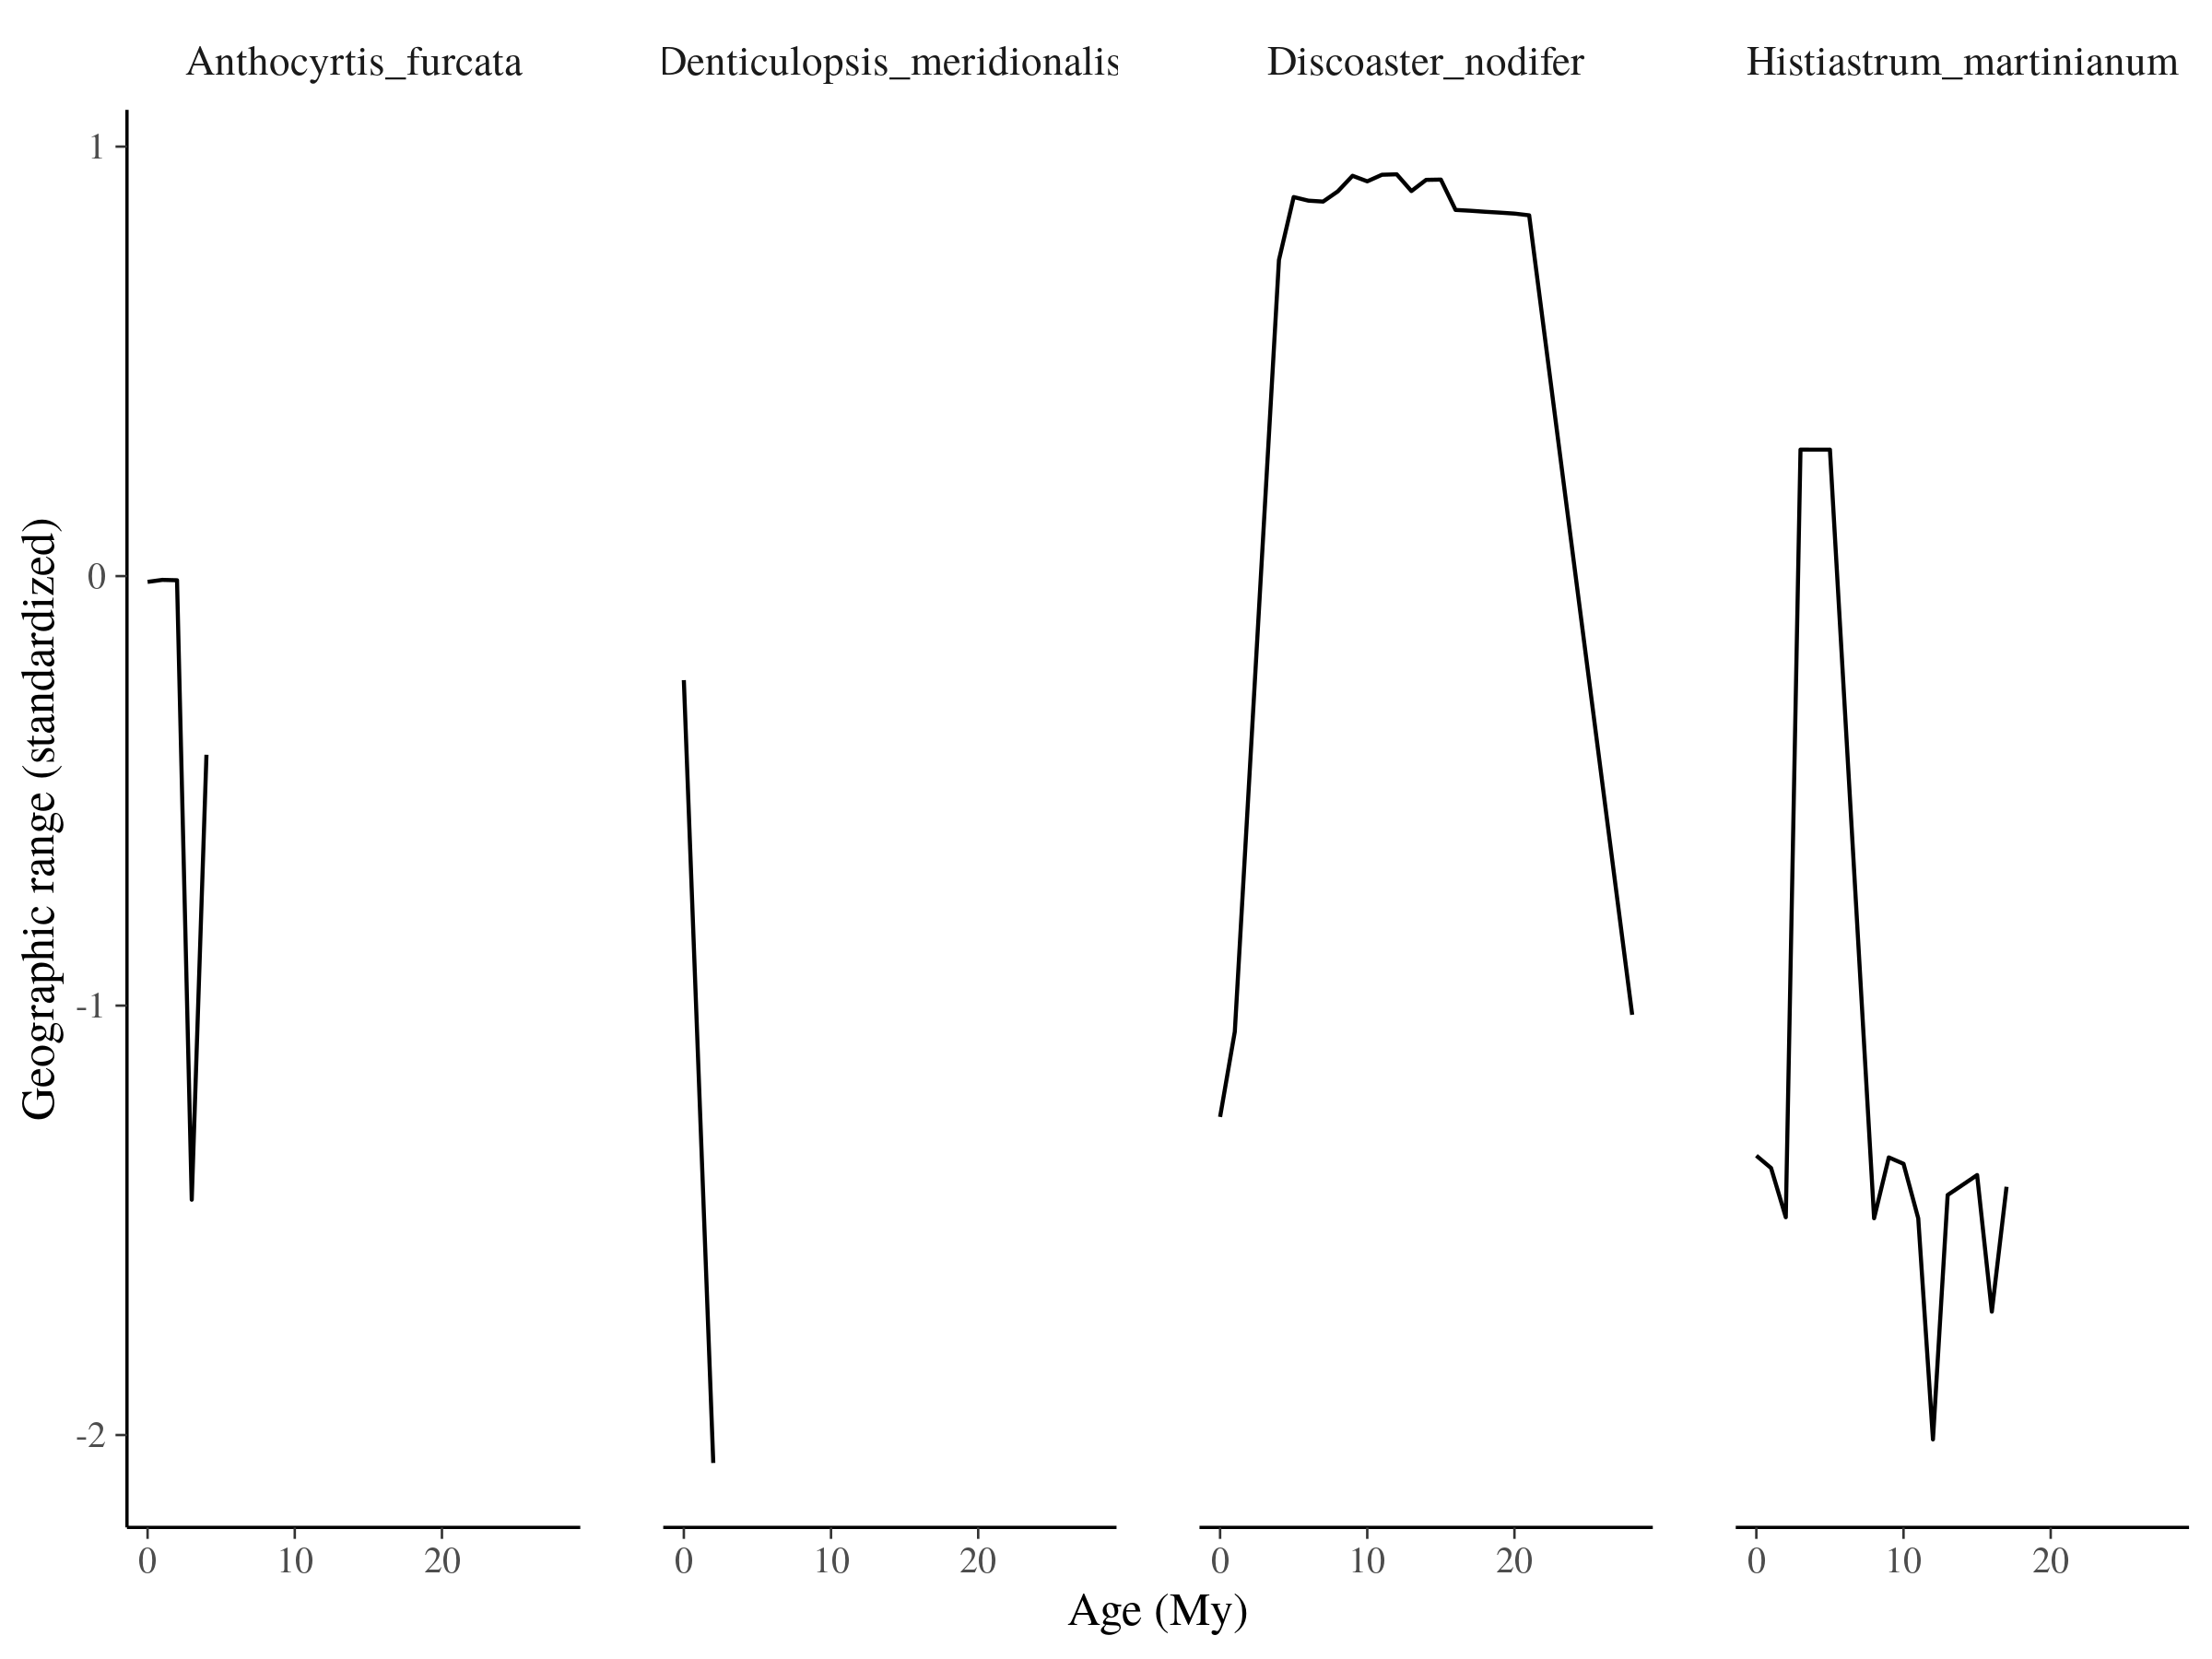
\includegraphics[width=\textwidth,height=0.5\textheight,keepaspectratio=true]{../results/figure/relrisk_range}
%  \caption{A}
%  \label{fig:relrisk_range}
% \end{subfigure}
%
% \begin{subfigure}{\textwidth}
%  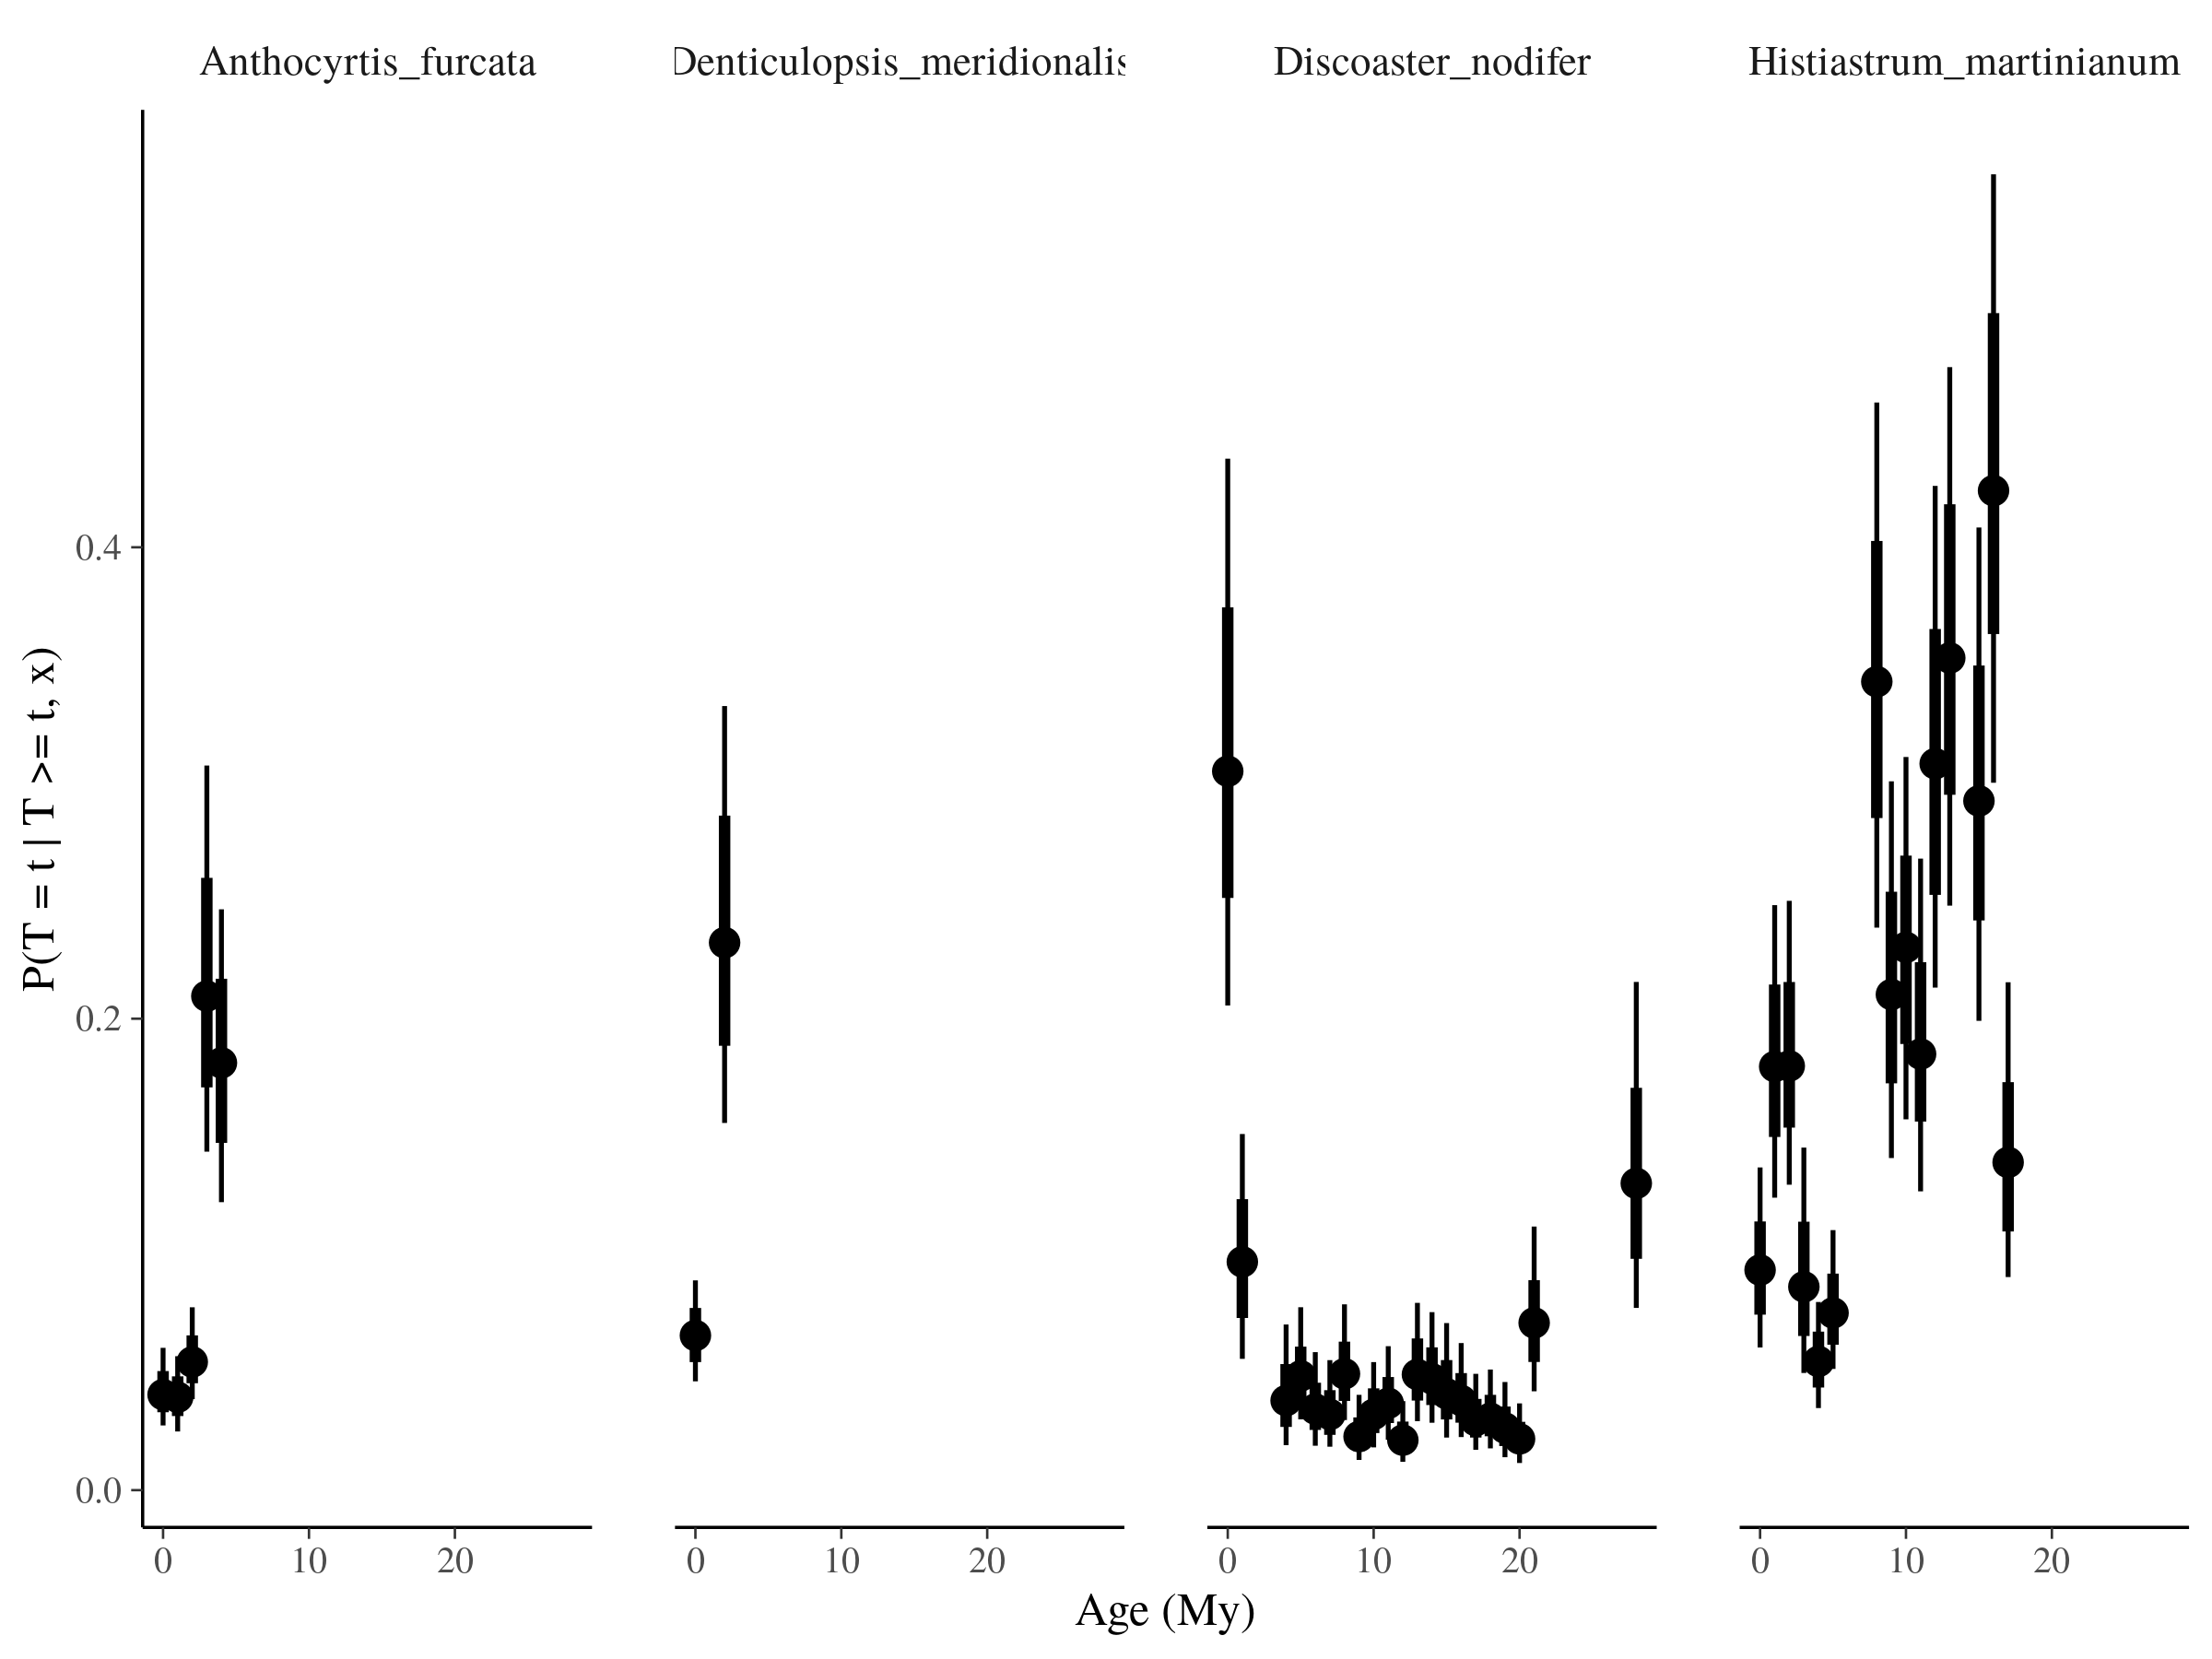
\includegraphics[width=\textwidth,height=0.5\textheight,keepaspectratio=true]{../results/figure/relrisk_ext}
%  \caption{B}
%  \label{fig:relrisk_ext}
% \end{subfigure}
% \caption{Comparison between species geographic range histories and our estimate of their probability of extinction for each time of observation. Geographic range is assumed observed without error. Our probability estimates are presented as a median (point) and 50\% and 80\% credible intervals.}
% \label{fig:relrisk_compare}
%\end{figure}



\section{Discussion}

We find that all of our models are expected to correctly forecasting the rank order in extinction probabilities for a randomly selected extinct-extant pair of future observations between 70\% to 80\% of the time (Fig. \ref{fig:fold_auc}). One of the most striking aspects of these results is the similarity in forecasting performance for in-sample and out-of-sample observations. A slight decrease in performance when dealing with out-of-sample observations makes sense: each of the models fit during cross-validation is based on fewer data than the model fit on the full data (between 1/5th to 4/5ths of the original). Additionally, a potential decrease in precision when forecasting the future of extinction risk is to be expected as the future will always differ from the past in some respect. However, the similarly between the in-sample and out-of-sample results indicates that our model is fairly robust to variation in extinction intensity over the Cenozoic. A extremely important caveat, of course, is that human impacts may substantially alter present and future extinction risk dynamics relative to the average Cenozoic state, so that the future may become less predictable than it has been in the past \citep{Harnik2012a,Finnegan2015}.

%This similarity demonstrates that while models with historical covariates are predictors of species extinction have better in-sample performance (Fig. \ref{fig:auc_hist}, \ref{fig:auc_taxon_time}), all of them forecast the extinction risk of out-of-sample data with a similar degree of success (Fig. \ref{fig:fold_auc}, \ref{fig:fold_auc_taxon_time}).

We also find that our four models are practically identical in their ability to make in-sample and out-of-sample forecasts. Although the in-sample AUC estimates differ between models, all of these estimates are in a narrow range of possible AUC values (Fig. \ref{fig:auc_hist}). While the ``best'' model does include the historical covariates and allows all covariate effects to vary over time, its practical difference in performance versus the other models is negligible (Fig. \ref{fig:fold_auc}). Thus even though the VP model has a statistically greater AUC for in-sample forecasts than the other three models, this result is not practically or scientifically significant. The results of the out-of-sample forecasts illustrate this point in full, as all four models have functionally identical out-of-sample performance. This including geographic range trajectory results in only very minor improvements in forecasting accuracy. This contrasts with findings from coral genera \citep{Kiessling2016} and suggests that further investigation of other taxa, timescales, and environments may help to elucidate the conditions under which past geographic range trajectories are most informative about future extinction risk.

%This result is an important reminder about understanding the practical interpretation of our analyses, which can be lost when we do not consider the predictive aspects of our analyses. By focusing on determining which covariates are ``significant'' and which model is best through simple comparisons means that the practical importance of the results are ignored. For example, in logistic regression a covariate can be considered significant on the log-odds scale but have no practical difference on the probability scale because the range of values is too small as to matter such as when the intercept is greater than 2 or less than -2 because the inverse-logit of those values are close to 0 or 1, respectively \citep{ARM}.

The relative quality and consistency of our models out-of-sample forecasting performance is encouraging given that its estimates are based on very limited biological and environmental information about the taxa. Even our most complex models only account for a few simple aspects of geographic range, prior history, and taxonomy. The principal reason we were not able to include more biological information in our models is that we lack suitably detailed life history or ecological information for many marine micro- and nannoplankton. Foraminifera are an exception to this problem as aspects of life history, ecology, and physiology are known for many foram species \citep{Ezard2011}. However, comparable information does not exist all foram species, nor does this type of data exist for the other three taxonomic groups studied here. Further analyses including this type of information and focused more narrowly on the foraminifera may be informative. 

%It performs nearly as well at out-of-sample prediction (70-80\%), implying that determinants of extinction risk have varied only modestly through time. An important caveat is that human impacts may substantially disrupt range-risk dynamics so that the future will be less predictable than it has been in the past.

%This presents an interesting conundrum about how to improve upon our results. A simple hypothesis for how to improve upon our results is that if we were to include more biological information in our model, our estimates of species relative extinction risk would be improved. However, if we decrease the amount of data in our model, our results by definition decrease in their quality. For example, compare the results from our models fit using full in-sample dataset, and the results from the cross-validation where the fit to each fold is by definition based on less than full information.)

In summary, our results suggest that models trained on prior extinction/survival patterns do modestly well at predicting the relative extinction risk of two randomly selected species based on a small number of taxonomic, geographic, and historical predictors. Considering that conservation decisions are made based on a continuum of risk, from most to least, this means that our results are in the same language as how conservation resources are allocated. These results present an encouraging baseline for using the fossil record to predict future extinction. This suggests, that all else being equal, extending this model to include the information in modern risk assessments might actually do decently well at forecasting future extinctions.


\printbibliography
\end{refsection}
\clearpage

\beginsupplement
\begin{refsection}

%\section{Supplemental Figures}
 
\section{Supplement to Materials and Methods}

\subsection{Data Specifications} \label{sec:data_desc}

\subsubsection{Binning fossil occurrences}

The estimated age of each occurrence is based on the core-specific age-model that observation is from and can be overly precise. To alleviate this overprecision, we coarsened our temporal information in an effort to limit the effects of between-core heterogeneity in age. The occurrence histories of each species was then summarized as a series of binary codes indicating the presence or last occurrence of that species. For every occurrence of a species, except the last, that species existence and survival is recorded as a 0. The last occurrence of that species is considered the bin in which the taxon has gone extinct -- and is recorded as 1. This protocol means that we are reading the fossil record ``as written,'' a practice that is potentially dangerous as it is an overconfident statement of preservation and may be shortening the actual durations of the studied species \citep{Alroy2010,Alroy2000b,Alroy2014,Foote1997,Foote1999a,Foote2001,Foote1996e,Lloyd2012b,Marshall1995,Wang2016}. However, this practice is common with marine microfossil data due to their exceptional preservation rate \citep{Ezard2013,Ezard2016,Ezard2011,Liow2010}. In fact, with marine microfossils collected from cores a bigger problem may be over extending the duration of a species due to mixing and smearing within the cores \citep{Mekik2018,Broecker1999,Mekik2014,Peng1984}.


\subsubsection{Covariate transformation and standardization}

Prior to analysis, geographic range was then log-plus-one transformed and standardized by mean-centering the data and then dividing by the standard deviation of the distribution of geographic ranges. This standardization means that a regression coefficient associated with each covariate describes the change in extinction probability per change in standard deviation of that covariate, that coefficients associated with similarly standardized covariates will be directly comparable in magnitude, and that the intercept term corresponds to the expected value of the outcome at when geographic range is its average value \citep{ARM}. Change in geographic range between observations was measured from the standardized geographic range values and was not standardized separately.

Temperature was also transformed and standardized the in the same manner as geographic range. The change in temperature between an observation and its previous observation was measured from the standardized temperature values and was not standardized separately.


\subsection{Model Specifications} \label{sec:model_desc}

In survival analysis, the hazard function describes the instantaneous rate of extinction of a species given its age and covariate information. The hazard function is defined as the conditional probability of a species going extinct by the end of the \(t\)-th interval given that it survived up until \(t\) and the relevant covariate information \(X\) for all \(k\) 1 My intervals \citep{Tutz2016}. For the discrete time intervals \(T = 1, \cdots, k\), extinction is defined as \(T = t\). The discrete time hazard function is defined as
\begin{equation}
 \lambda(t | X) = P(T = t | T \geq t, X), \quad t = 1, \cdots, k.
 \label{eq:hazard}
\end{equation}

The hazard function (Eq. \ref{eq:hazard}) is easily reparameterized as a logistic regression by defining that \(\lambda(t | X) = h(\Theta)\) where \(h(.)\) is a logit inverse-link function and \(\Theta\) is the probability of a taxon going extinction during interval \(t\) \citep{Tutz2016}. \(h(\Theta)\) is then modeled as with any regression. In this case, we opted for a hierarchical/mixed-effects model with multiple non-nested varying intercepts and slopes \citep{ARM}.

Our covariates matrix \(X\) is a \(N \times D\) matrix where \(N\) is the total number of observations and \(D\) is the total number of covariates. The first column of \(X\) is entirely 1's as it corresponds to the intercept term in the regression model. The next two columns of \(X\) are two aspects of geographic range as continuous covariates: geographic range \(r\) during interval \(t\), and the difference \(d\) between the geographic range at \(t - 1\) and \(t\). Change in geographic range was calculated from the transformed and standardized geographic range values; this means that change in geographic range is in units of changes in standard deviations. The final two columns are two aspects of global temperature: mean temperature during interval \(t\), and the lag of mean temperature (i.e. mean temperature during interval \(t - 1\).) As with change to geographic range, the lag of temperature is based on the transformed and standardized temperature estimates. 

The matrix of time and phylum varying regression coefficients describing the effects of the covariates on a species' risk of extinction is called \(B\) -- a \(w\) by \(p\) matrix, were \(w\) is the number of time temporal intervals and \(p\) is the number of phyla. The elements of this matrix, the regression coefficients, are themselves modeled as being multivariate normally distributed with vector of means \(\alpha\) describing the average intercept and regression coefficient estimates of each phylum \(p\). These phylum averages are themselves modeled as multivariate normally distributed with mean vector \(\mu\) describing the overall average regression coefficients, including the intercept. \(\mu\) has length \(D\) and is ordered intercept, range coefficient, change in range coefficient, temperature coefficient, temperature lag coefficient.

The effect of species age on the log-odds of species extinction is modeled as a non-nested random intercept \(A\) \citep{Tutz2016}. This term describes how the log-odds of extinction varies along a species duration, and how this effect can differ between the phyla. \(A\) is a \(l\) by \(p\) matrix, where \(l\) is the age at observation of a species and \(p\) is its phylum. \(A\) is modeled as following a multivariate normal distribution with phylum means being the vector \(\delta\) and covariance matrix \(\Sigma_{A}\). The covariation between the elements of vector \(\delta\) are modeled as a multivariate normal distribution with a mean vector of all 0s and covariance matrix \(\Sigma_{\delta}\).

To complete the generative model, we need to assign final priors to the ``top-level'' parameters. In general, we favored weakly informative priors which help regularize our estimates. In the case of a regression coefficient, this means a Normal distribution with mean 0 and a standard deviation of 3. For our scale parameters (e.g. standard deviations), we used half-Cauchy distributed priors with heavy tails but the majority of probability density near 0.

Our top-level intercept was given a more diffuse prior than our regression coefficients, which reflects our greater degree of uncertainty about its value. Our top-level regression coefficient for the effect of geographic range was given an informative prior reflecting the overwhelming amount of evidence that species with a larger than average geographic range have a lower risk of extinction than species with an average or less than average geographic range. In the context of this analysis, this means that we are again using a weakly informative prior but instead of centering the density around -1 (i.e. larger than average geographic range decreases extinction risk).

Instead of assigning a prior distribution for each of the covariance matrices in the model, we instead decomposed the covariance matrices (e.g. \(\Sigma_{B}\)) which allows us to assign independent priors for the scale and correlation aspects of covariance. The scale parameters were assigned half-Cauchy priors as described above in the context of all other scale parameters. The correlation matrices were assigned LKJ priors each with shape parameter set to 1. This choice of shape parameter produces a uniform distribution over possible correlation matrices. These priors are also slightly more interpretable than other common prior distributions for covariance matrices such as the inverse-Wishart distribution. This approach to assigning priors to a covariance matrix is recommended by the Stan Manual \citep{StanManual}.

In total, our model can be expressed as: 
\begin{equation}
 \begin{aligned}
  t_{i} &\sim \text{Bernoulli}(\Theta) \\
  \Theta_{i} &= \text{logit}^{-1} (X_{i} B_{w[i], p[i]} + A_{l[i], p[i]}) \\
  B_{w, p} &\sim MVN(\alpha_{p}, \Sigma_{B}) \\
  \alpha_{p} &\sim MVN(\mu, \Sigma_{\alpha}) \\
  % double check this\dots is A MVN dist?
  A_{l, p} &\sim MVN(\delta_{p}, \Sigma_{A}) \\
  \delta_{p} &\sim \mathrm{N}(0, \sigma_{\delta}) \\
  \mu_{d} &\sim 
  \begin{cases}
   N(-2, 5) & \text{if } d = \text{intercept} \\
   N(-1, 1) & \text{if } d = \text{geo. range} \\
   N(0, 1) & \text{else } \\
  \end{cases} \\
  \delta &\sim N(0, 1) \\
  \Sigma_{B} &= diag(\tau_{B}) \Omega_{B} diag(\tau_{B}) \\
  \Sigma_{\alpha} &= diag(\tau_{\alpha}) \Omega_{\alpha} diag(\tau_{\alpha}) \\
  \Sigma_{A} &= diag(\tau_{A}) \Omega_{A} diag(\tau_{A}) \\
  \tau_{B} &\sim C^{+}(1) \\
  \tau_{\alpha} &\sim C^{+}(1) \\
  \tau_{A} &\sim C^{+}(1) \\
  \Omega_{B} &\sim LKJ(1) \\
  \Omega_{\alpha} &\sim LKJ(1) \\
  \Omega_{A} &\sim LKJ(1) \\
 \end{aligned}
 \label{eq:model}
\end{equation}
with \(i\) indexing the observation and bracket subscripts referencing the class of the \(i\)th observation where \(w[i]\) is the time of the \(i\)-th observation, \(p[i]\) is the phylum of the \(i\)-th observation, and \(d[i]\) is the age of the \(i\)-th observation. 


\subsection{Model Parameter Estimation} \label{sec:model_est}

We implemented our model (Eq. \ref{eq:model} using the \begin{texttt}rstanarm\end{texttt} package for the R programming language \citep{StanManual}. This package provides an interface to the Stan probabilistic programming language for writing hierarchical/mixed-effects models in native R. Posterior estimates were obtained through Hamiltonian Monte Carlo, using 2000 steps divided equally between warm-up and sampling. In order to prevent divergent transitions adapt delta was increased to 0.999999; all other HMC/NUTS sampling parameters were kept at the defaults for rstanarm 2.18.2 \citep{rstanarm}.

To implement our VP model in \begin{texttt}rstanarm\end{texttt}, where ``data'' is a data.frame object of all necessary data (response, covariates), is coded as:
\begin{verbatim}
form <- event ~ range + range_diff + temp + temp_lag + 
        (1 + range + range_diff + temp + temp_lag | mybin/phylum) + 
        (1 | age/phylum), 
stan_glmer(formula = form,
      data = data, 
      family = 'binomial',
      prior = normal(c(-1, 0, 0, 0), rep(1, 4), autoscale = FALSE), 
      prior_intercept = normal(-2, 5, autoscale = FALSE), 
      prior_aux = cauchy(0, 1, autoscale = FALSE), 
      chains = 4,
      thin = 4,
      adapt_delta = 0.999999)
\end{verbatim}

Similarly, our VP model can be implemented using the \begin{texttt}brms\end{texttt} Stan interface \citep{brms2017,brms2018} as:
\begin{verbatim}
priors <- c(set_prior('normal(-2, 5)', class= 'Intercept'),
      set_prior('normal(0, 1)', class = 'b'),
      set_prior('normal(-1, 1)', class = 'b', coef = 'range'),
      set_prior('cauchy(0, 1)', class = 'sd'),
      set_prior('lkj(1)', class = 'cor'))
form <- bf(event ~ range + range_diff + temp + temp_lag +
      (1 + range + range_diff + temp + temp_lag | mybin/phylum) +
      (1 | age/phylum))
brmfit <- brm(formula = form,
       data = data, 
       family = bernoulli(), 
       prior = priors,
       chains = 4, 
       thin = 4,
       control = list(adapt_delta = 0.999999)
\end{verbatim}

Posterior convergence was determined using the general and HMC-specific diagnostic criteria: scale reduction factor (\(\hat{R}\); target \(<1.1\)), effective sample size (eff; target value eff/steps \(<0.0001\)), number of samples that saturated the maximum trajectory length for avoiding infinite loops (treedepth; target value 0), sample divergence, and the energy Bayesian Fraction of Mission Information (E-BFMI; target value \(>0.2\)). For further explanation of these diagnostic criteria, see the Stan Manual \citep{StanManual}.


\printbibliography[title={Supplementary References}]
\end{refsection}

\end{document}

